\documentclass[preprint,12pt]{elsarticle}

% --- Language and Encoding Packages ---
\usepackage[utf8]{inputenc}
\usepackage[OT1,T5]{fontenc}
\usepackage[vietnamese]{babel}
\renewcommand{\labelitemi}{$\bullet$}
\renewcommand{\labelitemii}{$\circ$}

% --- Mathematical Packages ---
\usepackage{amsmath,amssymb,amsfonts}

% --- Table and Figure Formatting ---
\usepackage{booktabs}
\usepackage{graphicx}
\usepackage{subcaption}
\usepackage{float}
\usepackage{tikz}
\usetikzlibrary{shapes.geometric, arrows.meta, positioning}

% --- Hyperlinks and URLs ---
\usepackage{hyperref}
\usepackage{url}
\hypersetup{
    colorlinks=true,
    linkcolor=blue!80!black,
    citecolor=blue!80!black,
    urlcolor=teal!80!black
}

% --- Mathematical Macros (latex_template standard) ---
\newcommand{\R}{\mathbb{R}}
\newcommand{\E}{\mathbb{E}}
\newcommand{\Var}{\mathrm{Var}}
\newcommand{\IoU}{\mathrm{IoU}}

\journal{Báo cáo Kỹ thuật Viễn thám \& Xử lý ảnh}

\begin{document}

\begin{frontmatter}

\title{Phát hiện Vết Dầu Loang trên Ảnh SAR: Quy trình Kết hợp Lọc Đốm Thống kê, Phân đoạn Ứng viên và Học máy Phân loại theo Vùng}

\author[utc]{Nhóm Nghiên cứu Xử lý Ảnh SAR -- Đề tài 18}
\address[utc]{Trường Đại học Giao thông Vận tải (UTC), Hà Nội, Việt Nam}

% Section 1: Abstract
\begin{abstract}
Phát hiện vết dầu tràn trên biển từ ảnh Radar khẩu độ tổng hợp (SAR) đóng vai trò quan trọng trong giám sát môi trường hàng hải, song thường chịu tỷ lệ báo nhầm cao do nhiễu đốm và các vùng tối nền biển khi áp dụng phân ngưỡng đơn thuần. Nghiên cứu này xây dựng và đánh giá thực nghiệm một quy trình tuần tự hai giai đoạn trên ảnh SAR đơn kênh mức xám: (1) Tạo vùng ứng viên thông qua lọc thống kê cục bộ Lee ($7 \times 7, L = 4$) tính bằng Bảng tổng tích lũy $\mathcal{O}(HW)$, phân ngưỡng toàn cục Otsu và lọc diện tích $A_{\min} = 64$ pixels; (2) Trích xuất 8 đặc trưng vùng (4 hình học, 4 bức xạ/biên) kết hợp bộ phân loại máy học vectơ hỗ trợ tuyến tính (LinearSVM) tối ưu hóa hàm mất mát Squared-Hinge điều chuẩn $L_2$. Thực nghiệm được thiết lập trên bộ dữ liệu Refined Deep-SAR Oil Spill (SOS) với $2\,683$ ảnh huấn luyện, $671$ ảnh kiểm định và $839$ ảnh kiểm thử độc lập của Sentinel-1A (băng C), cùng $776$ ảnh kiểm thử ngoài cảm biến của ALOS PALSAR (băng L). Trên tập kiểm thử Sentinel-1A, so với cấu hình tạo ứng viên không dùng bộ phân loại (Object F1 $= 0.1220$, $14.89$ FP/ảnh), việc tích hợp LinearSVM giúp giảm $76.6\%$ số vùng báo nhầm xuống còn $3.48$ FP/ảnh trong khi giữ lại $97.8\%$ số đối tượng đúng của giai đoạn tạo ứng viên ($996/1\,018$ TP), nâng Object F1 lên $0.2805$ (95\% CI $[0.2652, 0.2980]$) và Pixel IoU tổng hợp đạt $0.6614$; khi áp dụng trực tiếp sang ALOS PALSAR, mô hình đạt Object F1 $= 0.3724$. Nghiên cứu đồng thời làm rõ ba giới hạn cốt lõi: hiện tượng trọng số Lee với tham số cố định $L \le 4$ suy biến về lọc trung bình hộp trên ảnh PNG đã qua làm mượt, nút cổ chai độ thu hồi tổng thể ($\text{Recall} = 0.3130$ trên $3\,182$ đối tượng tham chiếu) do bước phân ngưỡng Otsu toàn cục chi phối, và sự lệch pha cấu trúc giữa nhãn huấn luyện theo độ tinh khiết điểm ảnh với thước đo đánh giá đối tượng Hungarian $\IoU \ge 0.5$.
\end{abstract}

\begin{keyword}
Vết dầu loang \sep Radar khẩu độ tổng hợp (SAR) \sep Lọc thống kê cục bộ \sep Phân ngưỡng Otsu \sep Trích xuất đặc trưng vùng \sep LinearSVM \sep Bộ dữ liệu SOS.
\end{keyword}


\end{frontmatter}

% Section 2: Introduction
\section{Giới thiệu}
\label{sec:introduction}

Sự cố tràn dầu trên biển là một trong những thảm họa sinh thái và môi trường nghiêm trọng nhất, đe dọa trực tiếp tới đa dạng sinh học biển, các rạn san hô, ngành đánh bắt thủy hải sản và kinh tế du lịch ven biển~\cite{fingas2014review}. Điển hình là các sự cố tràn dầu quy mô lớn trong lịch sử như sự cố nổ giàn khoan Deepwater Horizon năm 2010 tại Vịnh Mexico làm rò rỉ hàng trăm triệu lít dầu thô, hay các vụ rò rỉ từ cơ sở hạ tầng dầu khí Al-Khafji năm 2017 tại Vịnh Ba Tư~\cite{zhu2022oil}. Đối với các quốc gia có bờ biển dài như Việt Nam, việc phát hiện sớm và khoanh vùng chính xác các vệt dầu loang ngoài khơi đóng vai trò quyết định trong việc triển khai các biện pháp ứng phó khẩn cấp và bảo vệ hệ sinh thái biển.

Trong công tác giám sát hàng hải diện rộng, Radar khẩu độ tổng hợp (Synthetic Aperture Radar - SAR) đặt trên vệ tinh (như Sentinel-1 của Cơ quan Vũ trụ Châu Âu ESA hay ALOS PALSAR của Cơ quan Thám hiểm Hàng không Vũ trụ Nhật Bản JAXA) là công cụ viễn thám ưu việt nhất hiện nay nhờ khả năng chụp ảnh chủ động xuyên mây, hoạt động liên tục cả ngày lẫn đêm và không phụ thuộc vào điều kiện thời tiết hay ánh sáng mặt trời~\cite{brekke2005oil,topouzelis2008oil}. Cơ chế vật lý cơ bản của việc phát hiện vệt dầu trên ảnh SAR dựa trên sự tương tác giữa sóng điện từ và mặt biển: lớp màng dầu mỏng nổi trên bề mặt làm tăng độ nhớt động học, dập tắt các sóng mao dẫn và sóng trọng lực ngắn (sóng Bragg) do gió tạo ra. Hiện tượng này làm phẳng mặt biển cục bộ, khiến bức xạ radar bị phản xạ gương ra khỏi hướng thu của anten vệ tinh, dẫn đến cường độ tán xạ ngược (backscatter) bị suy giảm mạnh. Do đó, các vệt dầu thường xuất hiện dưới dạng các vùng tối (dark formations) nổi bật trên nền biển xung quanh~\cite{yang2025oil}.

Tuy nhiên, việc tự động hóa quá trình phát hiện vệt dầu loang từ ảnh SAR đối mặt với ba thách thức kỹ thuật lớn:
\begin{enumerate}
    \item \textbf{Nhiễu đốm nhân (Multiplicative Speckle Noise):} Do bản chất tạo ảnh giao thoa kết hợp của sóng radar, ảnh SAR luôn bị bao phủ bởi nhiễu đốm hạt có độ lệch chuẩn tỷ lệ thuận với cường độ tín hiệu, làm nhòe biên và gây dao động mức xám dữ dội, khiến các thuật toán phân ngưỡng thông thường dễ bị vỡ hạt và sinh hàng loạt đốm vụn giả mạo~\cite{lee1980digital}.
    \item \textbf{Các vùng tối giả mạo trên biển (Dark Formations / False Positives):} Các hiện tượng tự nhiên như vùng biển lặng gió (vận tốc gió $< 2-3\text{ m/s}$ không đủ kích hoạt sóng mao dẫn), màng hữu cơ sinh học do tảo biển tiết ra, dòng chảy nội hay vùng đổ bóng mưa cũng làm suy giảm tán xạ ngược, tạo ra các vùng tối có độ tương phản mức xám tương tự vệt dầu loang~\cite{brekke2005oil,solberg2007oil}.
    \item \textbf{Sự biến động quy mô diện tích và hình học:} Vết dầu trên biển có thể tồn tại dưới dạng dải hẹp phân mảnh chỉ vài pixel cho đến những mảng loang khổng lồ bao trọn toàn bộ khung ảnh viễn thám, gây khó khăn cho các phương pháp phân ngưỡng đơn lẻ.
\end{enumerate}

Để giải quyết các thách thức trên với một kiến trúc nhẹ, trong suốt và có thể diễn giải về mặt vật lý, nghiên cứu này xây dựng và đánh giá thực nghiệm một quy trình xử lý ảnh tuần tự kết hợp lọc đốm thống kê, phân đoạn ứng viên và học máy phân loại theo vùng (Sequential Statistical Filtering, Candidate Thresholding, and Region Classification Pipeline). Các đóng góp chính của nghiên cứu gồm:
\begin{itemize}
    \item Thiết kế và hiện thực hóa một quy trình tuần tự 2 giai đoạn (6 khối chức năng) hoàn chỉnh, độc lập với nhãn tham chiếu ground truth trong suy luận, kết hợp lọc thống kê cục bộ, phân ngưỡng Otsu, lọc diện tích và học máy phân loại giám sát.
    \item Cài đặt và kiểm chứng số học nghiêm ngặt toàn bộ pipeline bằng thư viện mảng NumPy thuần (đạt sai số tuyệt đối $< 10^{-11}$ và độ đồng thuận nhãn $100\%$ so với SciPy và scikit-learn), tính toán thống kê mô-men cục bộ bậc một và bậc hai thông qua Bảng tổng tích lũy với chi phí $\mathcal{O}(HW)$ độc lập với kích thước cửa sổ.
    \item Xây dựng không gian 8 đặc trưng vùng (4 đặc trưng hình học và 4 đặc trưng bức xạ/biên) giúp cắt giảm $76.6\%$ số vùng báo nhầm sinh ra sau phân ngưỡng (từ $14.89$ xuống $3.48$ FP/ảnh) trong khi giữ lại $97.8\%$ số đối tượng đúng của giai đoạn tạo ứng viên ($996/1\,018$ TP ứng viên).
    \item Thực hiện khảo sát thực nghiệm có kiểm soát trên lưới tham số quy mô lớn (110 cấu hình lọc/ngưỡng và 729 cấu hình mô hình vùng) trên tập kiểm định độc lập ($671$ ảnh Sentinel-1), chỉ rõ cơ chế suy biến của bộ lọc Lee về lọc trung bình hộp khi tham số cố định $L \in \{1, 4\}$ thấp hơn số looks hiệu dụng thực tế ($\text{ENL}$) của ảnh PNG đã qua tiền xử lý.
    \item Thẩm định khách quan theo giao thức ghép cặp đối tượng Hungarian ở ngưỡng $\IoU \ge 0.5$ và phân tầng theo 5 chế độ diện tích ($R_0 \to R_4$) trên tập kiểm thử độc lập $839$ ảnh Sentinel-1A và $776$ ảnh ALOS PALSAR, phân rã rõ hai nguồn lỗi trong chỉ số FP (báo nhầm thực sự trên nền biển sạch $\mathrm{Purity} \le 0.05$ và lỗi phân mảnh trên vùng dầu thật $\mathrm{Purity} \ge 0.5$) cũng như nút cổ chai độ thu hồi do bước phân ngưỡng toàn cục quyết định.
\end{itemize}


% Section 3: Related Work
\section{Nghiên cứu liên quan}
\label{sec:related_work}

Các nghiên cứu phát hiện vết dầu loang từ ảnh viễn thám SAR trong hơn ba thập kỷ qua tập trung vào ba chủ đề kỹ thuật cốt lõi: khử nhiễu đốm SAR, phân đoạn tách vùng tối ứng viên, và trích xuất đặc trưng kết hợp phân loại nhằm phân biệt vệt dầu với các vùng tối nền biển~\cite{fingas2014review,brekke2005oil}.

\subsection{Khử nhiễu đốm trên ảnh SAR}
Nhiễu đốm xuất hiện do hiện tượng giao thoa sóng tán xạ kết hợp từ vô số mục tiêu tán xạ thứ cấp phân bố ngẫu nhiên trong mỗi ô phân giải (resolution cell). Do đó, nhiễu đốm là nhiễu nhân chứ không phải nhiễu cộng: $I(x, y) = R(x, y) \cdot u(x, y)$, trong đó $R$ là độ phản xạ thực và $u$ là thành phần nhiễu ngẫu nhiên tuân theo phân phối Gamma~\cite{lee1980digital}. Các bộ lọc không gian tuyến tính kinh điển như lọc trung bình (Mean filter) hay lọc trung vị (Median filter) thường làm mờ đường biên của vệt dầu và xóa nhòa các dải hẹp~\cite{fingas2014review}.

Để khắc phục nhược điểm này, các bộ lọc thích nghi dựa trên thống kê cục bộ được phát triển, tiêu biểu là bộ lọc sai số toàn phương trung bình tối thiểu (MMSE) của Lee~\cite{lee1980digital}, bộ lọc Frost~\cite{frost1982model}, bộ lọc Kuan~\cite{kuan1985adaptive} và bộ lọc Gamma-MAP~\cite{lopes1990structure}. Bộ lọc Lee tính toán trọng số làm mịn thích nghi dựa trên tỷ số giữa phương sai cục bộ và mức nhiễu ước lượng: tại các vùng biển đồng nhất (phương sai thấp), bộ lọc tăng cường làm mịn để triệt tiêu đốm; ngược lại, tại các vùng biên ranh giới dầu--biển (phương sai cao), trọng số tiến dần về 1 để giữ lại giá trị ảnh gốc. Tuy nhiên, trên các sản phẩm SAR đã qua tiền xử lý đa góc nhìn (multi-look) hoặc chuẩn hóa mức xám về định dạng 8-bit, thống kê nhiễu nhân lý thuyết có thể bị thay đổi, khiến việc áp dụng cố định tham số số looks $L$ cần được kiểm chứng thực nghiệm cẩn trọng~\cite{brekke2005oil}.

\subsection{Phân ngưỡng và tách vùng tối ứng viên}
Sau khi làm mượt nhiễu đốm, bước tiếp theo là phân đoạn các vùng tán xạ thấp. Phương pháp phân ngưỡng toàn cục Otsu~\cite{otsu1979threshold} là kỹ thuật kinh điển nhờ tốc độ tính toán nhanh trên biểu đồ mức xám (histogram) và khả năng tối ưu hóa phương sai giữa hai lớp. Tuy nhiên, Otsu ngầm định histogram có dạng hai đỉnh (bimodal), dẫn đến nguy cơ chia đôi ảnh sai lệch khi tỷ lệ vết dầu chiếm phần quá nhỏ ($< 5\%$, chế độ $R_1$) hoặc khi khung ảnh ngập trọn vệt dầu lớn ($> 95\%$, chế độ $R_4$)~\cite{solberg2007oil}.

Để thích ứng với sự thay đổi cường độ nền biển trên diện rộng, các thuật toán phân ngưỡng cục bộ thích nghi như Niblack~\cite{niblack1986introduction} và Sauvola~\cite{sauvola2000adaptive} tính toán ngưỡng động cho từng điểm ảnh dựa trên trung bình và độ lệch chuẩn cục bộ trong cửa sổ trượt lân cận. Dù vậy, tại các vùng biển đồng nhất, ngưỡng cục bộ dễ bị hạ thấp và kích hoạt các điểm ảnh ở đuôi phân phối nhiễu thành các đốm tối giả mạo. Do đó, việc kết hợp hậu xử lý hình thái học (như lọc diện tích thành phần liên thông $A_{\min}$) và gán nhãn liên thông (Connected Component Labeling) là bắt buộc để hình thành các đối tượng vùng ứng viên có ý nghĩa vật lý trước khi phân loại~\cite{topouzelis2008oil}.

\subsection{Trích xuất đặc trưng và Phân loại vùng}
Để phân biệt giữa vệt dầu thật và các vùng tối giả mạo trên biển sinh ra từ hiện tượng biển lặng gió hay màng hữu cơ tự nhiên, các nghiên cứu nền tảng của Fiscella và cộng sự~\cite{fiscella2000oil}, Brekke \& Solberg~\cite{brekke2005oil}, Solberg và cộng sự~\cite{solberg2007oil}, Topouzelis~\cite{topouzelis2008oil} và Singha và cộng sự~\cite{singha2013oil} đã đề xuất không gian đặc trưng đa chiều trích xuất trên từng vùng ứng viên. Các đặc trưng này kết hợp cả tính chất hình học (diện tích, độ thuôn dài, độ đặc, độ phức tạp đường biên) và tính chất bức xạ/biên (độ tương phản giữa vùng tối và vành đai nền biển xung quanh, gradient biên).

Về giải thuật phân loại, các mô hình học máy truyền thống như Cây quyết định CART~\cite{breiman1984classification} và Máy học vectơ hỗ trợ (SVM)~\cite{cortes1995support} được sử dụng rộng rãi nhờ tính minh bạch, tốc độ suy luận nhanh và khả năng kiểm soát quá khớp tốt trên không gian đặc trưng kích thước nhỏ. Gần đây, các kiến trúc học sâu như mạng giám sát ngữ cảnh và biên CBD-Net của Zhu và cộng sự~\cite{zhu2022oil} (công trình giới thiệu bộ dữ liệu SOS) hay mạng phân đoạn của Krestenitis và cộng sự~\cite{krestenitis2019oil} đã đạt được độ chính xác phân đoạn điểm ảnh ấn tượng. Tuy nhiên, các mạng nơ-ron sâu đòi hỏi tài nguyên tính toán lớn (GPU chuyên dụng) và khó diễn giải tường minh quy tắc quyết định. Một quy trình tuần tự kết hợp xử lý ảnh thống kê và học máy phân loại theo vùng, được cài đặt và kiểm chứng số học chặt chẽ bằng thư viện mảng NumPy, cung cấp một đường cơ sở (baseline) nhẹ, rõ ràng và có thể kiểm chứng độc lập cho bài toán giám sát dầu tràn viễn thám.


% Section 4: Methodology
\section{Phương pháp nghiên cứu}
\label{sec:methodology}

Hệ thống phát hiện vết dầu loang trên ảnh SAR được xây dựng dưới dạng quy trình tuần tự 2 giai đoạn (6 khối chức năng), chuyển đổi từ ảnh thô đơn kênh mức xám $I \in [0, 1]^{H \times W}$ sang mặt nạ nhị phân dự đoán $\hat{M} \in \{0, 1\}^{H \times W}$. Quá trình suy luận hoạt động độc lập hoàn toàn, không sử dụng bất kỳ nhãn tham chiếu ground truth nào. Sơ đồ kiến trúc tổng quan của hệ thống được minh họa trên Hình~\ref{fig:pipeline_overview}.

\begin{figure}[!t]
\centering
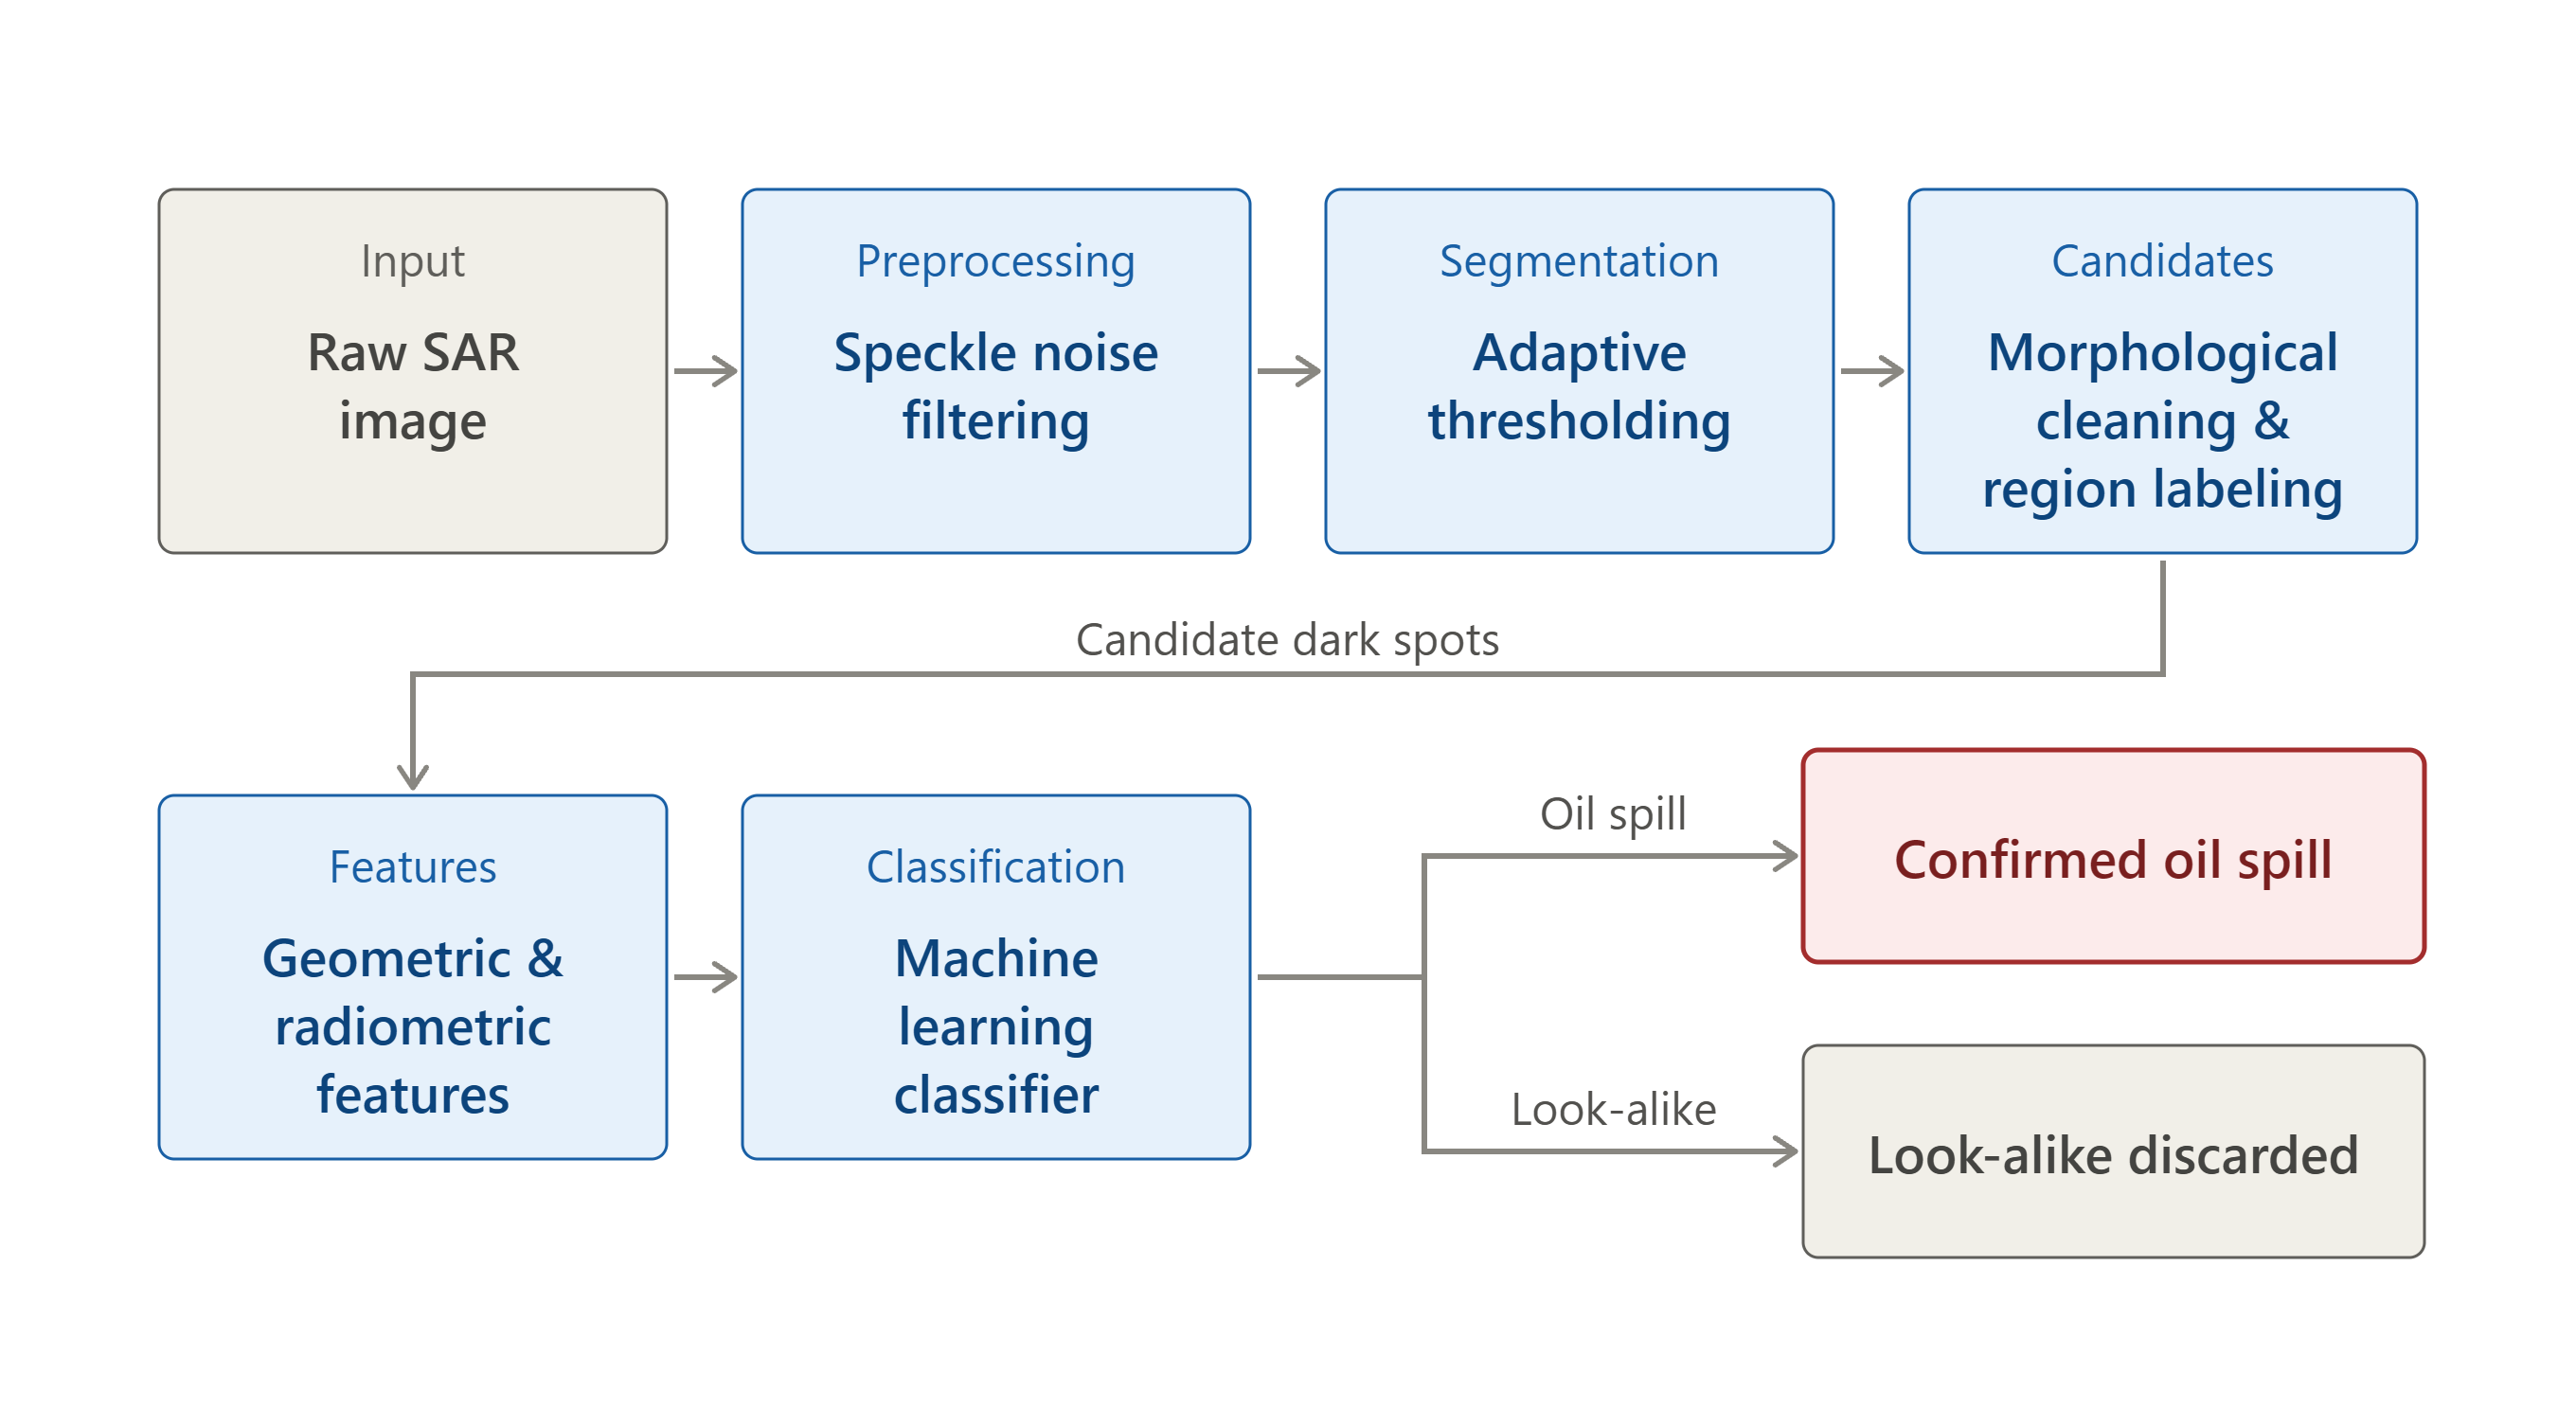
\includegraphics[width=0.95\linewidth]{figures/sar_oil_spill_detection_pipeline.png}
\caption{Sơ đồ khối kiến trúc tổng quan 2 giai đoạn của quy trình phát hiện vết dầu loang. Khối phân ngưỡng (\textit{Segmentation}) khảo sát ngưỡng tự động toàn cục Otsu $T^*$ (cấu hình chính) và ngưỡng thích nghi cục bộ Niblack; khối hậu xử lý thực hiện lọc diện tích $A_{\min} = 64$ pixels và gán nhãn liên thông 8 hướng; nhánh loại bỏ (\textit{Look-alike discarded}) trên bộ dữ liệu nhị phân SOS tương ứng với việc bác bỏ các vùng tối báo nhầm ($\hat{y}_i = 0$).}
\label{fig:pipeline_overview}
\end{figure}

\subsection{Khử nhiễu đốm bằng bộ lọc thống kê cục bộ Lee tối ưu hóa O(HW)}
\label{subsec:lee_filter}
Trên ảnh SAR cường độ tuyến tính thô, nhiễu đốm tuân theo mô hình thống kê nhân:
\begin{equation}
I(x, y) = R(x, y) \cdot u(x, y)
\end{equation}
trong đó $R(x, y)$ là hệ số phản xạ vô tuyến thực tế và $u(x, y)$ là thành phần nhiễu nhân có kỳ vọng $\mathbb{E}[u] = 1$, phương sai $\Var(u) = \sigma_u^2 = 1/L$ ($L$ là số looks tương đương của cảm biến).

Bộ lọc sai số toàn phương trung bình tối thiểu (Lee MMSE) xấp xỉ tuyến tính hóa hệ số phản xạ tại từng điểm ảnh thông qua trung bình cục bộ $m(x, y)$ và phương sai cục bộ $v(x, y)$:
\begin{equation}
\hat{R}(x, y) = m(x, y) + W(x, y) \cdot [I(x, y) - m(x, y)]
\label{eq:lee_formula}
\end{equation}
trong đó trọng số thích nghi $W(x, y) \in [0, 1]$ được xác định theo hệ số biến thiên cục bộ $C_I^2(x, y) = v(x, y) / m(x, y)^2$:
\begin{equation}
W(x, y) = \max\left(0, \frac{v(x, y) - \frac{m(x, y)^2}{L}}{\max(v(x, y), 10^{-12})}\right) = \max\left(0, 1 - \frac{1/L}{C_I^2(x, y)}\right)
\label{eq:lee_weight}
\end{equation}
Cấu hình chuẩn được khảo sát với kích thước cửa sổ $7 \times 7$, tham số $L \in \{1, 4\}$, và cơ chế đệm biên đối xứng (reflect padding). Cần lưu ý một đặc điểm quan trọng về miền giá trị dữ liệu: các ảnh trong bộ dữ liệu SOS được cung cấp dưới định dạng PNG 8-bit mức xám (chuẩn hóa tuyến tính về $[0, 1]$ bằng phép chia cho $255$) sau khi đã qua tiền xử lý khử đốm và nén dải động bởi nhà phát hành, chứ không còn ở miền công suất bức xạ $\sigma^0$ tuyến tính thuần túy. Do ảnh đã được làm trơn sơ bộ, số looks tương đương hiệu dụng thực tế trên các vùng biển đồng nhất ($\text{ENL}_{\text{eff}} = m^2 / v$) lớn hơn rất nhiều so với các giá trị danh định $L \in \{1, 4\}$. Hệ quả là điều kiện $C_I^2(x, y) \le 1/L$ (tức $v(x, y) \le m(x, y)^2/L$) xảy ra trên đại đa số điểm ảnh, làm cho trọng số $W(x, y) = 0$ và bộ lọc Lee với $L \le 4$ suy biến về bộ lọc trung bình hộp cục bộ $m(x, y)$.

\noindent\textbf{Tính toán mô-men cục bộ qua Bảng tổng tích lũy (Summed-Area Table):}
Ảnh mức xám được ép kiểu sang số thực độ chính xác kép 64-bit (\texttt{float64}) trên miền $[0, 1]$ nhằm tránh triệt tiêu số học. Chúng tôi xây dựng hai bảng tích phân hai chiều:
\begin{equation}
S(y, x) = \sum_{j \le y, i \le x} I(j, i), \quad S_2(y, x) = \sum_{j \le y, i \le x} I^2(j, i)
\end{equation}
Sau khi khởi tạo $S$ và $S_2$ với chi phí $\mathcal{O}(HW)$, giá trị trung bình $m(x, y)$ và trung bình bình phương $\mathbb{E}[I^2]$ trong bất kỳ cửa sổ hình chữ nhật kích thước $(2r+1) \times (2r+1)$ nào đều được tính toán trong thời gian $\mathcal{O}(1)$ thông qua 4 phép truy vấn góc:
\begin{equation}
\Sigma = S(y+r, x+r) - S(y-r-1, x+r) - S(y+r, x-r-1) + S(y-r-1, x-r-1)
\end{equation}
Phương sai cục bộ được tính có kẹp dưới không âm: $v(x, y) = \max(\mathbb{E}[I^2] - m(x, y)^2, 0)$. Nhờ đó, phép lọc thống kê cục bộ được hoàn tất với chi phí tính toán tuyến tính theo số điểm ảnh $\mathcal{O}(HW)$, hoàn toàn độc lập với bán kính cửa sổ lọc $r$.

\subsection{Phân đoạn tạo vùng ứng viên: Phân ngưỡng Otsu và Niblack}
\label{subsec:otsu_threshold}
Do hiện tượng làm phẳng sóng mao dẫn biển của vệt dầu, vùng dầu có cường độ tán xạ ngược thấp hơn nền biển. Thuật toán phân ngưỡng toàn cục Otsu chia biểu đồ mức xám (histogram) 256 bin của ảnh sau lọc $I_f$ thành hai lớp $\omega_0$ (vùng tối) và $\omega_1$ (nền biển) tại ngưỡng $t \in [0, 1]$ bằng cách tối đa hóa phương sai giữa hai lớp:
\begin{equation}
t^* = \arg\max_{t} \sigma_B^2(t), \quad \sigma_B^2(t) = \omega_0(t)\omega_1(t) [\mu_0(t) - \mu_1(t)]^2
\label{eq:otsu_between}
\end{equation}
trong đó $\omega_0(t), \omega_1(t)$ là xác suất tích lũy của hai lớp, và $\mu_0(t), \mu_1(t)$ là cường độ trung bình tương ứng. Mặt nạ nhị phân thô được xác định bởi:
\begin{equation}
B(x, y) = [I_f(x, y) < t^*]
\end{equation}
Đồng thời, tỷ số phương sai $\eta = \sigma_B^2(t^*) / \sigma_T^2 \in [0, 1]$ ($\sigma_T^2$ là tổng phương sai ảnh) được ghi nhận để chẩn đoán mức độ phân tách của histogram.

Đối với phân ngưỡng cục bộ Niblack trong cửa sổ trượt $W$, mặt nạ được xác định bởi:
\begin{equation}
B_{\text{Niblack}}(x, y) = [I_f(x, y) < m_W(x, y) - k \cdot s_W(x, y)]
\label{eq:niblack_formula}
\end{equation}
với $m_W, s_W$ là trung bình và độ lệch chuẩn cục bộ tính qua bảng tích lũy, và $k > 0$ là hệ số điều chỉnh (tương ứng với hệ số âm $-k$ trong ký hiệu chuẩn Niblack cho đối tượng tối trên nền sáng).

\subsection{Hậu xử lý diện tích và Gán nhãn liên thông 8 hướng}
\label{subsec:morphology_cca}
Để triệt tiêu các đốm nhiễu hạt nhỏ còn sót lại trên mặt biển mà không làm biến dạng biên vệt dầu, quy trình áp dụng ngưỡng diện tích thành phần liên thông tối thiểu $A_{\min} = 64$ pixels:
\begin{equation}
B_{\text{clean}} = \bigcup \{ \Omega_k \subset B \mid |\Omega_k| \ge A_{\min} \}
\end{equation}
Sau đó, mặt nạ nhị phân $B_{\text{clean}}$ được gán nhãn thành $K$ vùng ứng viên độc lập $\{\Omega_1, \Omega_2, \dots, \Omega_K\}$ bằng thuật toán Run-Length Union-Find 8 hướng với kỹ thuật nén đường đi (path compression).

\subsection{Không gian 8 đặc trưng vùng vật lý và xử lý ca biên}
\label{subsec:features}
Với mỗi vùng ứng viên $\Omega_i$ ($i = 1, \dots, K$), hệ thống trích xuất vector đặc trưng $\mathbf{x}_i = [f_0, f_1, \dots, f_7]^T \in \mathbb{R}^8$, bao gồm 4 đặc trưng hình học và 4 đặc trưng bức xạ/biên như được định nghĩa chi tiết trong Bảng~\ref{tab:features}.

\begin{table*}[!t]
\centering
\caption{Định nghĩa toán học và ý nghĩa vật lý của 8 đặc trưng vùng trích xuất cho mỗi thành phần liên thông $\Omega_i$.}
\label{tab:features}
\resizebox{\textwidth}{!}{%
\begin{tabular}{clclp{7.2cm}}
\toprule
\textbf{Ký hiệu} & \textbf{Tên đặc trưng} & \textbf{Nhóm} & \textbf{Công thức toán học} & \textbf{Ý nghĩa vật lý} \\
\midrule
$f_0$ & \texttt{area\_fraction} & Hình học & $A_i / (H \cdot W)$ & Tỷ lệ diện tích vùng so với diện tích toàn bộ khung ảnh viễn thám ($256 \times 256$ pixels). \\
$f_1$ & \texttt{elongation} & Hình học & $\sqrt{\frac{\lambda_2 + 10^{-6}}{\lambda_1 + 10^{-6}}}$ & Độ thuôn dài, tính từ hai trị riêng $\lambda_1 \le \lambda_2$ của ma trận hiệp phương sai tọa độ vùng. \\
$f_2$ & \texttt{extent} & Hình học & $A_i / (W_{\text{bbox}} \cdot H_{\text{bbox}})$ & Tỷ lệ lấp đầy của vùng so với diện tích hộp bao ngoài chữ nhật. \\
$f_3$ & \texttt{complexity} & Hình học & $P_i^2 / (4\pi A_i)$ & Độ phức tạp đường biên, với chu vi lưới $P_i$ đếm cạnh chuyển tiếp pixel. \\
\midrule
$f_4$ & \texttt{mean} & Bức xạ & $\mu_i = \frac{1}{A_i}\sum_{(x,y) \in \Omega_i} I_f(x, y)$ & Cường độ phản xạ SAR trung bình bên trong vùng ứng viên. \\
$f_5$ & \texttt{std} & Bức xạ & $\sigma_i = \sqrt{\frac{1}{A_i}\sum_{(x,y) \in \Omega_i} (I_f - \mu_i)^2}$ & Độ biến thiên cường độ mức xám nội vùng. \\
$f_6$ & \texttt{boundary\_gradient} & Biên & $\frac{1}{|\partial \Omega_i|}\sum_{(x,y) \in \partial \Omega_i} \|\nabla I_f(x, y)\|$ & Độ dốc biên trung bình: Sobel chuẩn hóa trên vành biên trong $\partial \Omega_i = \Omega_i \setminus (\Omega_i \ominus B_1)$. \\
$f_7$ & \texttt{background\_contrast} & Tương phản & $\frac{\mu_{\mathrm{bg}} - \mu_i}{|\mu_{\mathrm{bg}}| + 10^{-6}}$ & Độ tương phản bức xạ giữa vành đai nền biển 5 pixel ngoài biên và cường độ nội vùng. \\
\bottomrule
\end{tabular}%
}
\end{table*}

\noindent\textbf{Cơ chế xử lý ca biên, tính chất tự tham chiếu của nền và lý do loại trừ đặc trưng kết cấu:}
Khi trích xuất đặc trưng cho vùng $\Omega_i$:
\begin{enumerate}
    \item Hộp bao cục bộ được mở rộng thêm lề 5 pixel $[y_{\min}-5 : y_{\max}+6, x_{\min}-5 : x_{\max}+6]$ và kẹp chặt trong biên khung ảnh $[0, H) \times [0, W)$.
    \item Chu vi lưới $P_i$ và biên trong $\partial \Omega_i$ được tính toán trên mảng đệm ngoại vi bằng \texttt{False}, đảm bảo các cạnh tiếp giáp mép ảnh được tính chính xác vào chu vi và biên.
    \item Vành đai nền biển 5 pixel được xác định bởi $(\Omega_i \oplus B_5) \cap \{ \text{labels} == 0 \}$, chỉ lấy điểm ảnh ngoài vùng ứng viên. Cần lưu ý hai đặc tính cấu trúc của định nghĩa này: (a) Do tập hợp $\{\text{labels} == 0\}$ chủ yếu bao gồm các điểm ảnh có mức xám $\ge t^*$ (cùng một số đốm tối nhỏ $< A_{\min}$ vừa bị loại bỏ), giá trị $\mu_{\text{bg}}$ mang thiên lệch sáng có cấu trúc và phụ thuộc một phần vào chính ngưỡng Otsu $t^*$ (đặc trưng mang tính ``tự tham chiếu''); (b) Trong các khung cảnh ngập dầu diện rộng ($R_3/R_4$), khi ngưỡng Otsu buộc phải chia đôi chính mảng dầu đơn đỉnh hoặc khi vành đai 5 pixel rỗng khiến thuật toán chuyển sang nhánh dự phòng (fallback: tính $\mu_{\text{bg}}$ trên $I_f[\text{labels} == 0]$ hoặc trung bình toàn ảnh), tập $\{\text{labels} == 0\}$ thực chất lại là phần dầu sáng hơn. Khi đó, độ tương phản $f_7$ bị suy giảm mạnh một cách hệ thống, có thể khiến bộ phân loại bác bỏ nhầm vùng dầu thật.
    \item Khác với một số công trình kinh điển sử dụng ma trận đồng xuất hiện mức xám (GLCM)~\cite{brekke2005oil,singha2013oil}, nghiên cứu này không đưa nhóm đặc trưng kết cấu Haralick vào vector $\mathbf{x}_i$ vì hai lý do: (a) Ảnh PNG 8-bit trong bộ dữ liệu SOS đã qua làm mượt tiền xử lý khiến cấu trúc hạt vi mô bị triệt tiêu đáng kể, phần biến thiên mức xám nội vùng đã được đại diện bởi $f_5 = \sigma_i$; (b) Việc lượng tử hóa và tích lũy ma trận đồng xuất hiện 2 chiều theo nhiều hướng trên từng vùng liên thông có hình dạng bất kỳ làm tăng mạnh độ trễ khi một ảnh có hàng chục ứng viên.
\end{enumerate}

\subsection{Gán nhãn huấn luyện, Cân bằng lớp và Độ lệch với thước đo đánh giá}
\label{subsec:training_labels}
Trong giai đoạn huấn luyện, nhãn giám sát $y_i \in \{0, 1\}$ của từng vùng ứng viên được gán tự động dựa trên độ tinh khiết điểm ảnh (pixel purity) so với mặt nạ tham chiếu ground truth $G$:
\begin{equation}
\mathrm{Purity}(\Omega_i) = \frac{|\Omega_i \cap G|}{|\Omega_i|}
\end{equation}
Quy tắc gán nhãn phân tách:
\begin{itemize}
    \item \textbf{Vết dầu thật ($y_i = 1$):} $\mathrm{Purity}(\Omega_i) \ge 0.50$.
    \item \textbf{Vùng tối báo nhầm ($y_i = 0$):} $\mathrm{Purity}(\Omega_i) \le 0.05$.
    \item \textbf{Vùng biên trung gian ($0.05 < \mathrm{Purity} < 0.50$):} Loại bỏ khỏi tập huấn luyện để tránh nhiễu ranh giới quyết định.
\end{itemize}

Trên $2\,683$ ảnh huấn luyện Sentinel-1A, bước tạo ứng viên sinh ra tổng cộng $39\,530$ vùng ứng viên, gồm $11\,092$ vùng dương ($28.1\%$), $25\,946$ vùng âm ($65.6\%$) và $2\,492$ vùng trung gian ($6.3\%$). Để xử lý mất cân bằng lớp, chúng tôi áp dụng kỹ thuật lấy mẫu giảm ngẫu nhiên (undersampling) với seed cố định $2026$, chọn tối đa $10\,000$ mẫu mỗi lớp, tạo thành tập huấn luyện cân bằng gồm đúng $20\,000$ mẫu ($10\,000$ dương, $10\,000$ âm, tương ứng loại bỏ khoảng $61.5\%$ mẫu âm). Các đặc trưng được chuẩn hóa Z-score dựa trên kỳ vọng và độ lệch chuẩn $(\mu_k, \sigma_k)$ tính riêng trên tập huấn luyện:
\begin{equation}
z_{i,k} = \frac{x_{i,k} - \mu_k}{\max(\sigma_k, 10^{-12})}, \quad k = 0, \dots, 7
\end{equation}

\noindent\textbf{Sự khác biệt cấu trúc giữa nhãn huấn luyện (Purity) và thước đo đánh giá (Object IoU):}
Cần nhấn mạnh rằng $\mathrm{Purity}(\Omega_i) = |\Omega_i \cap G| / |\Omega_i|$ chuẩn hóa theo diện tích của riêng mảnh ứng viên $|\Omega_i|$, trong khi thước đo đánh giá cuối cùng ($\mathrm{IoU} = |\hat{\Omega}_p \cap G_q| / |\hat{\Omega}_p \cup G_q| \ge 0.50$) chuẩn hóa theo diện tích hợp với đối tượng tham chiếu nguyên khối $G_q$. Do đó, khi một vết dầu lớn $G_q$ bị bước phân ngưỡng Otsu cắt vụn thành nhiều mảnh nhỏ nằm trọn trong lòng vết dầu, mỗi mảnh đều có $\mathrm{Purity} = 1.0$ (nên bộ phân loại học cách giữ lại chúng như mẫu dương hợp lệ), nhưng từng mảnh riêng lẻ lại có $\mathrm{IoU} < 0.50$ so với $G_q$ (hoặc bị dư thừa do ràng buộc ghép cặp 1-1) và bị quy thành False Positive (FP) ở bước đánh giá đối tượng.

\subsection{Bộ phân loại LinearSVM với Tối ưu hóa Gradient Nesterov và CART}
\label{subsec:linearsvm}
Mô hình Linear Support Vector Machine tối ưu hóa hàm mục tiêu lồi có điều chuẩn $L_2$ trên toàn bộ vector trọng số $\mathbf{w} \in \mathbb{R}^9$ (gồm 8 trọng số đặc trưng và 1 hệ số chặn bias ở vị trí cuối) với hàm mất mát Squared-Hinge Loss:
\begin{equation}
\min_{\mathbf{w}} J(\mathbf{w}) = \frac{1}{2n}\|\mathbf{w}\|_2^2 + \frac{C}{n}\sum_{i=1}^n \max\left(0, 1 - y_i^* (\mathbf{z}_i^T \mathbf{w})\right)^2
\label{eq:svm_objective}
\end{equation}
trong đó $y_i^* = 2y_i - 1 \in \{-1, +1\}$, $\mathbf{z}_i = [z_{i,0}, \dots, z_{i,7}, 1]^T$, $n = 20\,000$ là số lượng mẫu huấn luyện, và $C = 10.0$ là siêu tham số phạt vi phạm lề.

Do hàm Squared-Hinge khả vi liên tục bậc một, gradient của $J(\mathbf{w})$ xác định bởi:
\begin{equation}
\nabla J(\mathbf{w}) = \frac{1}{n}\mathbf{w} - \frac{2C}{n}\sum_{i \in \mathcal{V}} y_i^* (1 - y_i^* \mathbf{z}_i^T \mathbf{w})\mathbf{z}_i
\end{equation}
với $\mathcal{V} = \{i \mid 1 - y_i^* \mathbf{z}_i^T \mathbf{w} > 0\}$ là tập các mẫu vi phạm lề. Bài toán được tối ưu hóa bằng thuật toán Nesterov Accelerated Gradient (NAG) với kỹ thuật tìm bước nhảy quay lui (backtracking line search) và tự động thiết lập lại xung lượng (adaptive restart). Điều kiện dừng hội tụ được áp dụng trên hàm mục tiêu đã chia trung bình cho $n = 20\,000$:
\begin{equation}
\|\nabla J(\mathbf{w})\|_\infty \le 10^{-6}
\end{equation}
(tương đương chuẩn vô cùng của gradient tổng chưa chia $n$ đạt $\approx 0.02$; tính hội tụ sát cực tiểu toàn cục được kiểm chứng trực tiếp đối chiếu với bộ giải chuẩn của \texttt{scikit-learn}, đạt độ lệch giá trị hàm mục tiêu $|J_{\text{NumPy}}^* - J_{\text{sklearn}}^*| = 2.88 \times 10^{-12}$ và đồng thuận dự đoán $100\%$). Vùng ứng viên $\Omega_i$ được phân loại là vết dầu loang tại ngưỡng quyết định cố định $\mathbf{z}_i^T \mathbf{w} > 0$.

Song song với LinearSVM, mô hình Cây quyết định CART được khảo sát làm mô hình đối sánh với tiêu chuẩn phân tách tạp chất Gini, độ sâu tối đa $\text{max\_depth} = 3$ và số mẫu tối thiểu tại nút lá $\text{min\_leaf} = 20$.


% Section 5: Experiments
\section{Thiết lập thực nghiệm}
\label{sec:experiments}

\subsection{Bộ dữ liệu chuẩn Refined Deep-SAR Oil Spill (SOS)}
\label{subsec:dataset}
Nghiên cứu sử dụng bộ dữ liệu công khai Deep-SAR Oil Spill (SOS), được giới thiệu bởi Zhu và cộng sự~\cite{zhu2022oil} và chuẩn hóa trên kho lưu trữ Zenodo~\cite{zuenko2025refined}. Bộ dữ liệu được xây dựng từ 21 cảnh ảnh vệ tinh SAR thô bao phủ hai khu vực xảy ra thảm họa tràn dầu lớn:
\begin{enumerate}
    \item \textbf{Vịnh Mexico (Sự cố tràn dầu Deepwater Horizon, năm 2010):} Bao gồm 14 cảnh ảnh thu nhận từ cảm biến ALOS PALSAR băng L (sản phẩm mức 1.5), độ phân giải lấy mẫu không gian $12.5\text{ m}$, kênh phân cực ngang-ngang (HH).
    \item \textbf{Vịnh Ba Tư (Khu vực mỏ dầu Al-Khafji, năm 2017):} Bao gồm 7 cảnh ảnh thu nhận từ cảm biến Sentinel-1A băng C ở chế độ quét rộng giao thoa (IW) mức 1 (GRD), độ phân giải không gian $5\text{ m} \times 20\text{ m}$, góc tới dao động từ $29.1^\circ$ đến $46^\circ$, kênh phân cực dọc-dọc (VV).
\end{enumerate}

\begin{table}[!t]
\centering
\caption{Thống kê cấu trúc phân chia bộ dữ liệu Refined Deep-SAR Oil Spill (SOS).}
\label{tab:dataset_stats}
\resizebox{\linewidth}{!}{%
\begin{tabular}{lcc}
\toprule
\textbf{Thuộc tính} & \textbf{Sentinel-1A (Vịnh Ba Tư)} & \textbf{ALOS PALSAR (Vịnh Mexico)} \\
\midrule
Cảm biến vệ tinh & Sentinel-1A & ALOS PALSAR \\
Băng tần radar & Băng C ($\sim 5.6\text{ cm}$) & Băng L ($\sim 23.6\text{ cm}$) \\
Kênh phân cực & VV & HH \\
Độ phân giải danh định & $5\text{ m} \times 20\text{ m}$ & $12.5\text{ m}$ \\
Sự cố tràn dầu & Al-Khafji (2017) & Deepwater Horizon (2010) \\
Số cảnh ảnh thô gốc & 7 cảnh & 14 cảnh \\
Kích thước patch chuẩn hóa & $256 \times 256$ pixels & $256 \times 256$ pixels \\
\midrule
Tập huấn luyện (Train) & $2\,683$ ảnh & Không sử dụng ($3\,101$ ảnh lưu kho) \\
Tập kiểm định (Validation) & $671$ ảnh & Không sử dụng \\
Tập kiểm thử (Test độc lập) & $839$ ảnh (thư mục \texttt{val} gốc) & $776$ ảnh (Test ngoài cảm biến, \texttt{val} gốc) \\
\midrule
\textbf{Tổng số mẫu ảnh sử dụng} & \textbf{4\,193 ảnh} & \textbf{776 ảnh} \\
\bottomrule
\end{tabular}%
}
\end{table}

\noindent\textbf{Giao thức phân chia dữ liệu và giới hạn cấp cảnh:}
Theo nhà phát hành bộ dữ liệu~\cite{zuenko2025refined}, 21 cảnh SAR gốc được cắt thành các mảnh nhỏ, tăng cường dữ liệu và chuẩn hóa về kích thước $256 \times 256$ pixels. Để đảm bảo tính liêm chính thực nghiệm, chúng tôi thiết lập giao thức phân chia 3 tập nghiêm ngặt (Bảng~\ref{tab:dataset_stats}):
\begin{itemize}
    \item $3\,354$ ảnh của tập huấn luyện gốc Sentinel-1A (\texttt{train/}) được phân chia theo tỷ lệ 80:20 (phân tầng theo ảnh rỗng và có dầu với seed $2026$) thành: \textbf{2\,683 ảnh Train} (dùng để trích xuất mẫu huấn luyện SVM/CART) và \textbf{671 ảnh Validation} (dùng độc quyền để sàng lọc 110 cấu hình lọc/ngưỡng và 729 cấu hình mô hình vùng).
    \item $839$ ảnh của phân tập kiểm định gốc Sentinel-1A (\texttt{val/} của nhà phát hành) được giữ nguyên làm \textbf{tập Test độc lập}, chỉ được mở khóa đánh giá một lần duy nhất cho cấu hình chiến thắng sau khi toàn bộ quy trình và mô hình đã được đóng băng.
    \item $776$ ảnh của phân tập \texttt{val/} gốc thuộc ALOS PALSAR được sử dụng làm \textbf{tập kiểm thử ngoài cảm biến} (out-of-sensor test) với mô hình đã đóng băng từ Sentinel-1A (không sử dụng $3\,101$ ảnh \texttt{train/} của PALSAR).
\end{itemize}
Cần lưu ý một giới hạn thực nghiệm quan trọng: do bộ dữ liệu công khai trên Zenodo không kèm định danh cảnh gốc (scene ID) hay tọa độ địa lý, việc phân chia được thực hiện ở cấp patch, do đó không thể bảo đảm tính độc lập tuyệt đối theo cảnh thô viễn thám ban đầu.

\noindent\textbf{Không gian tìm kiếm siêu tham số $110 \times 729$ và quy tắc lựa chọn:}
Quá trình lựa chọn mô hình trên $671$ ảnh Validation được tiến hành theo hai bước có kiểm soát:
\begin{enumerate}
    \item \textit{Sàng lọc bộ lọc và ngưỡng tạo ứng viên (110 cấu hình, cố định hình thái học \texttt{none} và $A_{\min} = 16$):} Kết hợp tích Đề-các giữa \textbf{11 bộ lọc} (\texttt{none}; \texttt{median} kích thước $\{3, 5\}$; \texttt{gaussian} với $\sigma \in \{0.8, 1.2\}$; \texttt{lee} với kích thước $\{3, 5, 7\} \times L \in \{1, 4\}$) và \textbf{10 bộ phân ngưỡng} (\texttt{otsu} toàn cục; \texttt{niblack} cục bộ với cửa sổ $\{15, 31, 51\} \times k \in \{0.2, 0.5, 0.8\}$).
    \item \textit{Tìm kiếm cấu hình hình thái, đặc trưng và bộ phân loại (729 cấu hình):} Giữ lại Top-3 cấu hình lọc/ngưỡng đầu bảng (Lee $7\times 7, L=4$ + Otsu; Lee $7\times 7, L=1$ + Otsu; Lee $5\times 5, L=4$ + Otsu) và quét toàn diện tích Đề-các: $3 \text{ (cấu hình lọc/ngưỡng)} \times 3 \text{ (phép hình thái $3\times 3$: \texttt{none, close, open\_close})} \times 3 \text{ (ngưỡng diện tích } A_{\min} \in \{4, 16, 64\}) \times 3 \text{ (nhóm đặc trưng: \texttt{shape, intensity, all})} \times 9 \text{ (mô hình: 6 cấu hình CART với } \text{max\_depth} \in \{3, 5, 8\} \times \text{min\_leaf} \in \{5, 20\} \text{ và 3 cấu hình LinearSVM với } C \in \{0.1, 1, 10\}) = 729$ tổ hợp.
    \item \textit{Quy tắc xếp hạng và thiên lệch lựa chọn:} Tại mỗi bước, các cấu hình nằm trong dải $\text{F1-band} = 0.005$ so với mức F1 cao nhất được ưu tiên xếp hạng theo độ thu hồi Recall giảm dần, sau đó theo thời gian chạy tăng dần. Việc chọn cấu hình đứng đầu từ 729 tổ hợp trên cùng tập Validation (671 ảnh) tất yếu mang lại một mức độ lạc quan do lựa chọn (selection optimism) đối với các con số trên Validation, do đó hiệu năng thực tế phải được phán quyết trên tập Test độc lập ($839$ ảnh).
\end{enumerate}

Mặt nạ nhị phân ground truth $G \in \{0, 1\}^{H \times W}$ được xác lập bằng ngưỡng chuẩn:
\begin{equation}
G(x, y) = [M_{\text{raw}}(x, y) \ge 128]
\end{equation}

\subsection{Giao thức phân tầng theo tỷ lệ diện tích dầu}
\label{subsec:regimes}
Dựa trên tỷ lệ diện tích dầu $r = \frac{1}{HW}\sum_{x, y} G(x, y)$, toàn bộ dữ liệu được phân tầng thành 5 chế độ diện tích:
\begin{itemize}
    \item \textbf{$R_0$ (Biển sạch):} $r = 0$, khung cảnh không chứa dầu, kiểm định tỷ lệ cảnh báo sai (False Alarm).
    \item \textbf{$R_1$ (Vết dầu nhỏ):} $0 < r < 0.05$, diện tích dầu dưới 5\% khung ảnh, mô phỏng các vết dầu mới rò rỉ.
    \item \textbf{$R_2$ (Vết dầu trung bình):} $0.05 \le r < 0.50$, bao gồm các dải dầu dài, hẹp hoặc bị phân mảnh.
    \item \textbf{$R_3$ (Vết dầu diện rộng):} $0.50 \le r < 0.95$, vệt dầu bao phủ phần lớn khung ảnh.
    \item \textbf{$R_4$ (Patch ngập dầu toàn phần):} $0.95 \le r \le 1.00$, khung ảnh nằm trọn trong vệt dầu lớn.
\end{itemize}

\begin{table}[!t]
\centering
\caption{Phân bố số lượng ảnh thực tế theo 5 chế độ diện tích ($R_0 \to R_4$) trên tập kiểm thử độc lập Sentinel-1A (839 ảnh) và tập kiểm thử ngoài cảm biến ALOS PALSAR (776 ảnh).}
\label{tab:regime_counts}
\resizebox{\linewidth}{!}{%
\begin{tabular}{lccccc}
\toprule
\textbf{Tập kiểm thử} & \textbf{$R_0$} & \textbf{$R_1$} & \textbf{$R_2$} & \textbf{$R_3$} & \textbf{$R_4$} \\
\midrule
Sentinel-1A Test (839 ảnh, \texttt{val/} gốc) & 31 & 99 & 457 & 196 & 56 \\
ALOS PALSAR Test ngoài cảm biến (776 ảnh, \texttt{val/} gốc) & 45 & 113 & 585 & 31 & 2 \\
\bottomrule
\end{tabular}%
}
\end{table}

\begin{figure*}[!t]
\centering
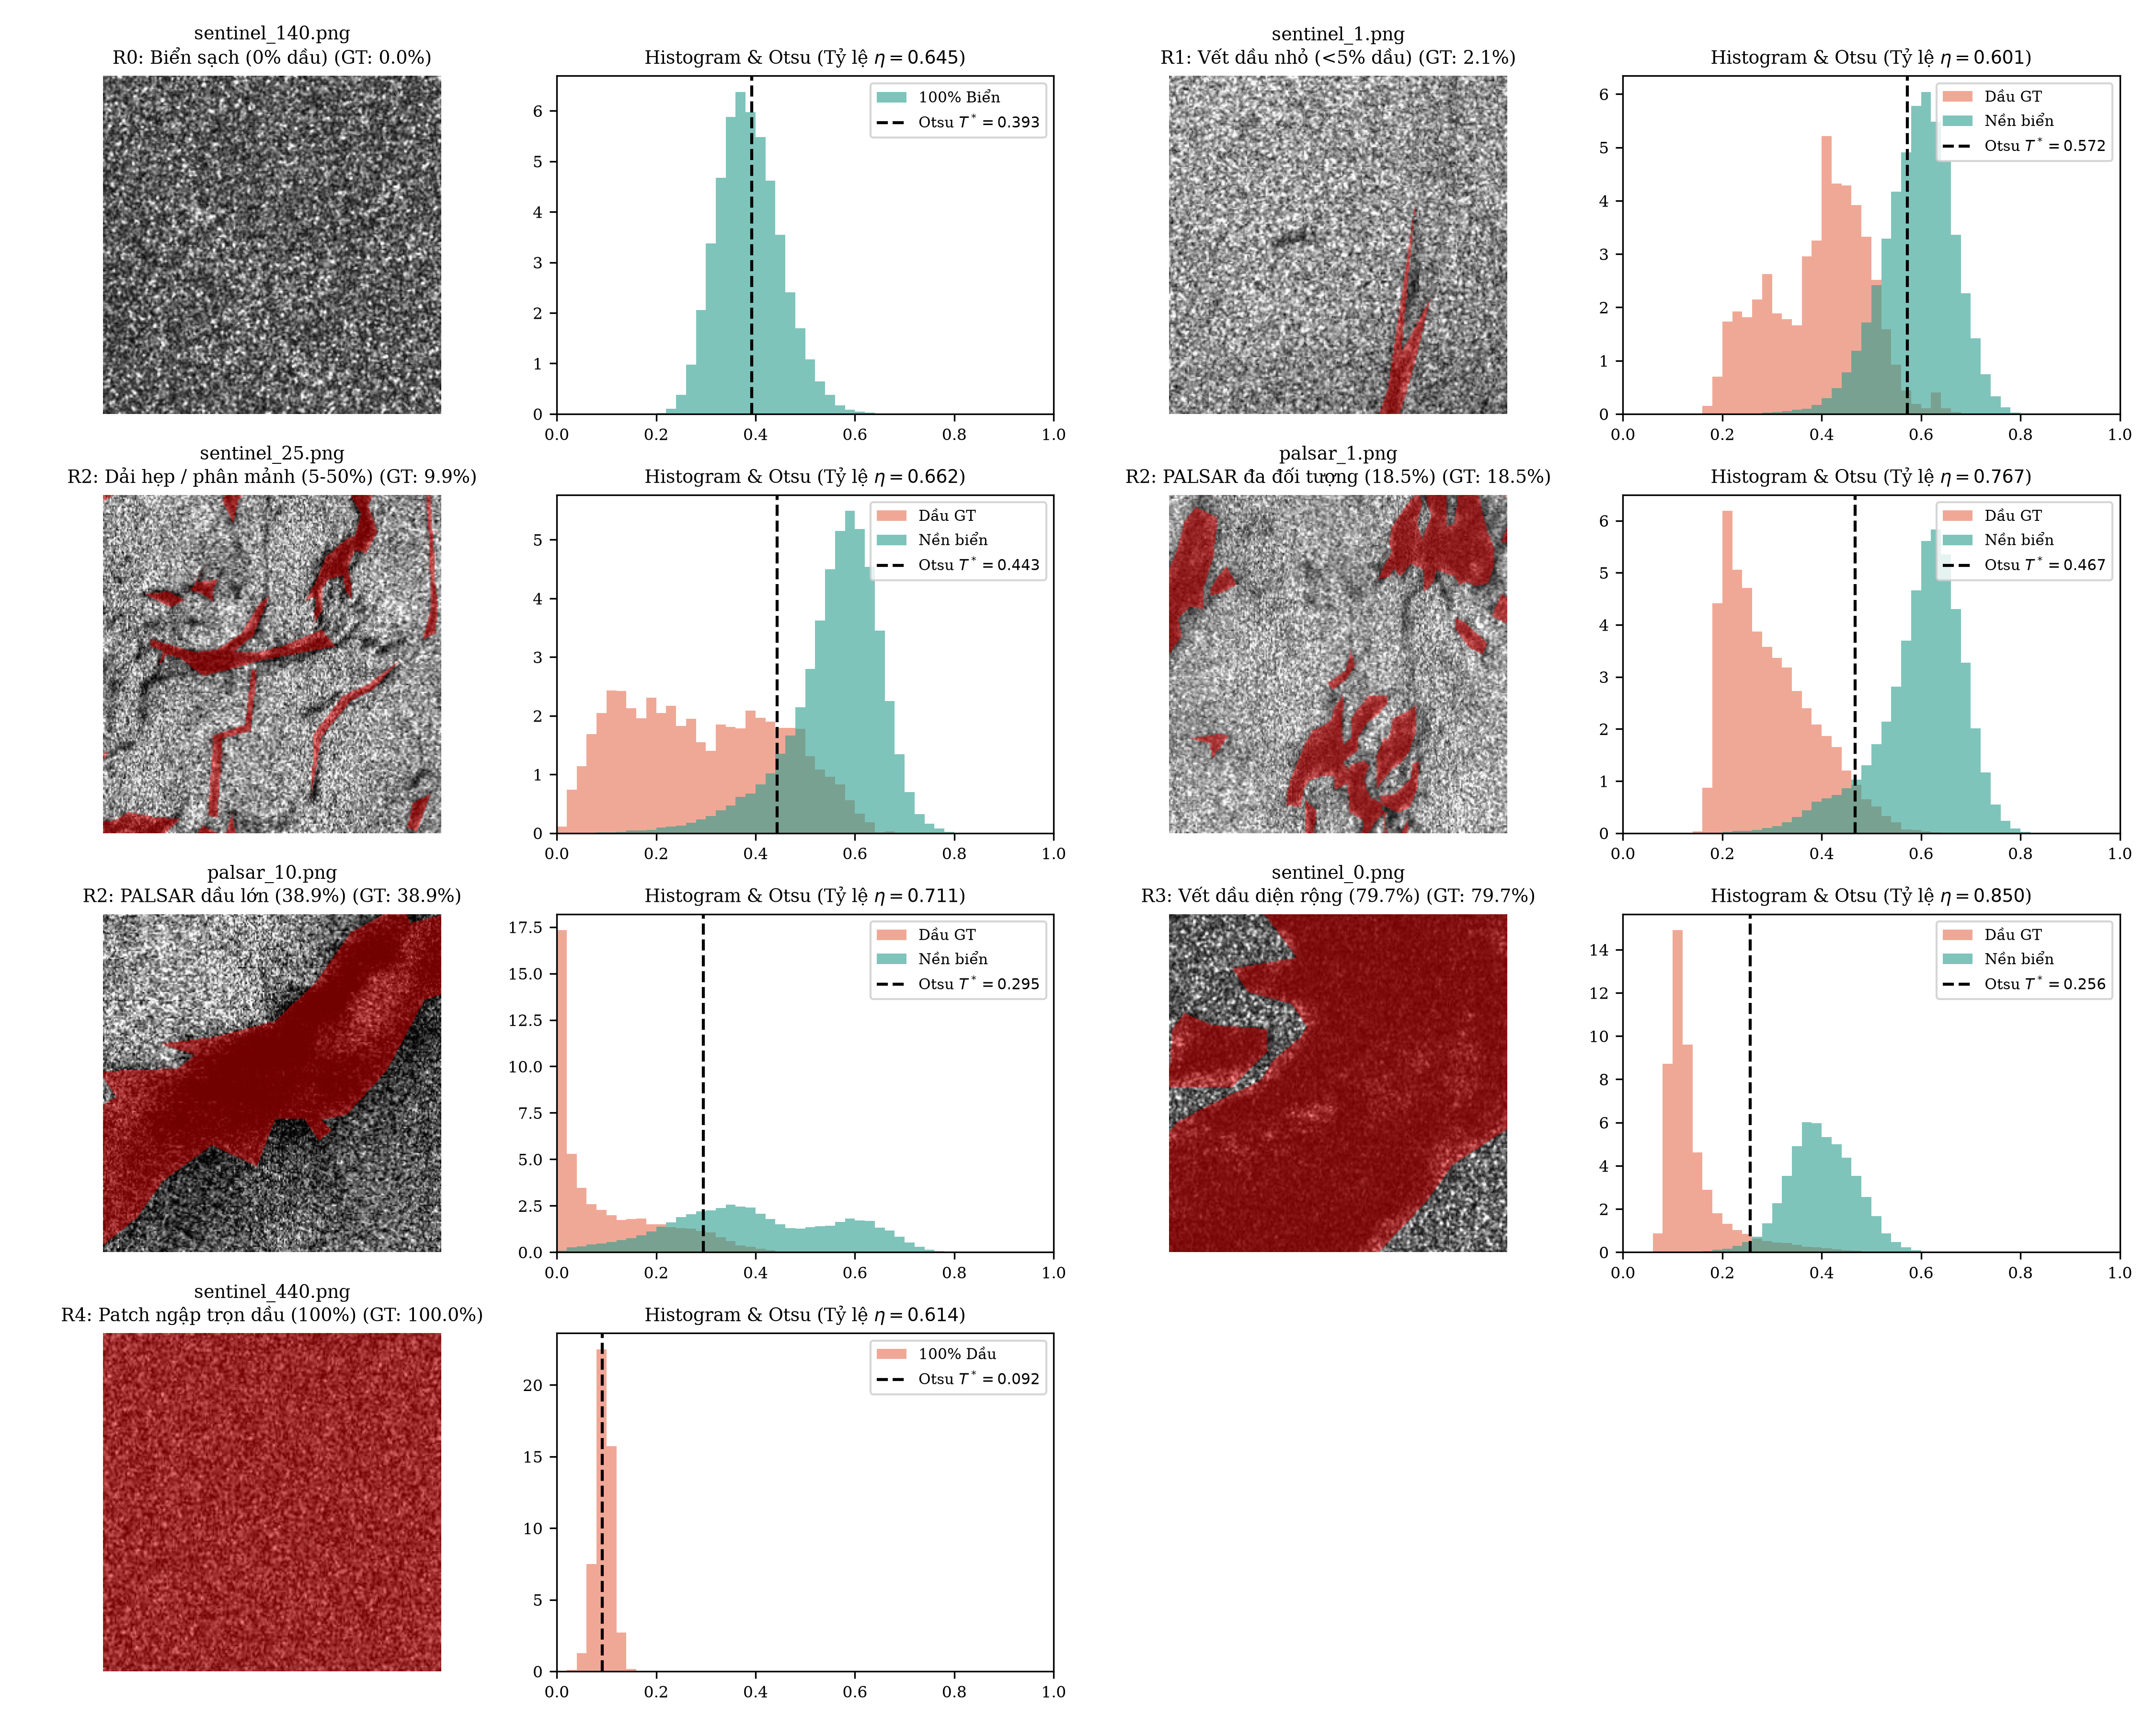
\includegraphics[width=\textwidth]{figures/fig2_sos_dataset_regimes.png}
\caption{Minh họa các mẫu ảnh SAR thực tế, mặt nạ Ground Truth và phân bố Histogram kèm ngưỡng Otsu $T^*$ và tỷ số phương sai $\eta = \sigma_B^2(T^*)/\sigma_T^2$ qua 5 chế độ diện tích dầu ($R_0 \to R_4$). Nguồn ảnh trích từ phân tập \texttt{val/} gốc của nhà phát hành SOS (tương ứng tập Test độc lập, chỉ dùng để minh họa định tính sau khi đã đóng băng mô hình): \texttt{sentinel\_140.png} ($R_0$), \texttt{sentinel\_1.png} ($R_1$), \texttt{sentinel\_25.png}, \texttt{palsar\_1.png}, \texttt{palsar\_10.png} ($R_2$), \texttt{sentinel\_0.png} ($R_3$) và \texttt{sentinel\_440.png} ($R_4$).}
\label{fig:sos_regimes}
\end{figure*}

Hình~\ref{fig:sos_regimes} minh họa các mẫu ảnh thực tế và biểu đồ histogram tương ứng, chỉ ra rằng phân bố hai đỉnh chỉ xuất hiện rõ ở các chế độ trung bình $R_2$, trong khi ở $R_0$ và $R_4$, histogram hoàn toàn đơn đỉnh khiến ngưỡng Otsu thô vẫn chia đôi ảnh. Bảng~\ref{tab:regime_counts} thống kê chi tiết số lượng ảnh trên hai tập kiểm thử, cho thấy sự khác biệt lớn về phân bố chế độ: ALOS PALSAR tập trung $75.4\%$ ($585/776$) ảnh ở chế độ trung bình $R_2$ và chỉ có $4.3\%$ ($33/776$) ở $R_3+R_4$, trong khi Sentinel-1A có tới $30.0\%$ ($252/839$) ảnh thuộc chế độ diện rộng $R_3+R_4$.

\subsection{Giao thức đánh giá đối tượng chuẩn Hungarian, Đánh giá điểm ảnh và Môi trường tái lập}
\label{subsec:metrics}
Nghiên cứu áp dụng đồng thời hai cấp độ đánh giá độc lập:

\noindent\textbf{1. Đánh giá cấp đối tượng theo thuật toán Hungarian ($\IoU \ge 0.5$):}
Mỗi mặt nạ dự đoán $\hat{M}$ và mặt nạ tham chiếu $G$ được phân rã thành các thành phần liên thông 8 hướng: $\hat{M} \to \{\hat{\Omega}_1, \dots, \hat{\Omega}_P\}$ và $G \to \{G_1, \dots, G_Q\}$. Ma trận chỉ số giao trên hợp (IoU) giữa từng cặp vùng có kích thước $P \times Q$:
\begin{equation}
\mathrm{IoU}_{p, q} = \frac{|\hat{\Omega}_p \cap G_q|}{|\hat{\Omega}_p \cup G_q|}
\end{equation}
Bài toán ghép cặp một-một tối ưu được giải bằng thuật toán Hungarian (Linear Sum Assignment) với điều kiện hợp lệ $\mathrm{IoU}_{p, q} \ge 0.5$. Một cặp $(p, q)$ được công nhận là True Positive (TP) khi và chỉ khi được ghép cặp thành công tại ngưỡng này. Mọi vùng dự đoán dư thừa bị tính là False Positive (FP), và mọi vùng ground truth bị bỏ sót bị tính là False Negative (FN).

Chúng tôi phân biệt rõ hai khái niệm:
\begin{itemize}
    \item \textbf{Candidate Object F1:} F1 cấp đối tượng tính trực tiếp trên các vùng ứng viên sinh ra từ giai đoạn 1 (trước khi phân loại).
    \item \textbf{Object F1 (Final):} F1 cấp đối tượng sau khi đã qua bộ phân loại học máy.
\end{itemize}

Bên cạnh cách tính cộng gộp vi mô (Micro-averaging) trên toàn bộ tập ảnh:
\begin{equation}
\text{Precision} = \frac{\sum \text{TP}}{\sum \text{TP} + \sum \text{FP}}, \quad \text{Recall} = \frac{\sum \text{TP}}{\sum \text{TP} + \sum \text{FN}}
\end{equation}
\begin{equation}
\text{Object F1} = \frac{2 \sum \text{TP}}{2 \sum \text{TP} + \sum \text{FP} + \sum \text{FN}}
\end{equation}
chúng tôi báo cáo thêm giá trị trung bình vĩ mô và độ lệch chuẩn giữa các ảnh (Macro-averaging: $\text{mean} \pm \text{SD}$, với $\text{ddof}=0$) trên các ảnh có mẫu số xác định ($\text{TP}+\text{FP}>0$ cho Precision, $\text{TP}+\text{FN}>0$ cho Recall, và $2\text{TP}+\text{FP}+\text{FN}>0$ cho F1; các ảnh biển sạch $R_0$ được lọc sạch hoàn toàn với $\text{TP}=\text{FP}=\text{FN}=0$ có mẫu số bằng $0$ được ghi nhận riêng số lượng $n$ xác định tại từng cột), cùng chỉ số \textbf{Edge Recall} (tỷ lệ thu hồi đối với các đối tượng GT chạm viền ảnh) và \textbf{Interior Recall} (đối tượng GT nằm trọn vẹn bên trong khung ảnh).

\noindent\textbf{2. Đánh giá cấp điểm ảnh (Pixel-level):}
Độ bao phủ không gian tổng hợp toàn tập được lượng hóa bởi:
\begin{equation}
\text{Pixel IoU} = \frac{\sum |\hat{M} \cap G|}{\sum |\hat{M} \cup G|}, \quad \text{Dice} = \frac{2 \sum |\hat{M} \cap G|}{\sum |\hat{M}| + \sum |G|}
\end{equation}
Đồng thời, chỉ số số lượng báo nhầm trung bình trên mỗi ảnh (\textbf{FP/ảnh}) được ghi nhận để đánh giá mức độ làm sạch đối với các vùng tối dư thừa.

\noindent\textbf{3. Thông số môi trường và chứng thực tái lập (Reproducibility Provenance):}
Toàn bộ thực nghiệm được khóa mã băm chứng thực trong \texttt{run\_manifest.json} và \texttt{evaluation.json}: thực thi trên Python \texttt{3.13.12} (Windows x86\_64, 4 tiến trình worker song song, cố định biến môi trường đơn luồng \texttt{OMP/MKL/OPENBLAS\_NUM\_THREADS=1}), sử dụng thư viện \texttt{numpy 2.5.4}, \texttt{scipy 1.18.1}, \texttt{scikit-image 0.26.0}, \texttt{scikit-learn 1.9.1}, \texttt{Pillow 13.0.0}, \texttt{matplotlib 3.11.2}, hằng số ngẫu nhiên \texttt{seed = 2026}, và mã băm kiểm kê dữ liệu \texttt{manifest\_sha256 = 572d38f21c25a628...c9bed7e}.


% Section 6: Results
\section{Kết quả thực nghiệm và thảo luận}
\label{sec:results}

\subsection{Khảo sát có kiểm soát các bộ lọc và phân ngưỡng tạo ứng viên}
\label{subsec:bench_filters}
Giai đoạn đầu tiên quyết định chất lượng của tập ứng viên $\{\Omega_i\}$: nếu bộ lọc không đủ mạnh, nhiễu đốm sẽ tạo ra hàng chục vùng vụn; ngược lại, nếu làm mượt quá mức, các dải dầu hẹp sẽ bị xóa nhòa. Chúng tôi tiến hành khảo sát thực nghiệm có kiểm soát 13 cấu hình lọc không gian kết hợp phân ngưỡng toàn cục Otsu (cố định ngưỡng diện tích $A_{\min} = 16$ pixels) trên toàn bộ $671$ ảnh thuộc tập kiểm định (Validation).

\begin{figure*}[!t]
\centering
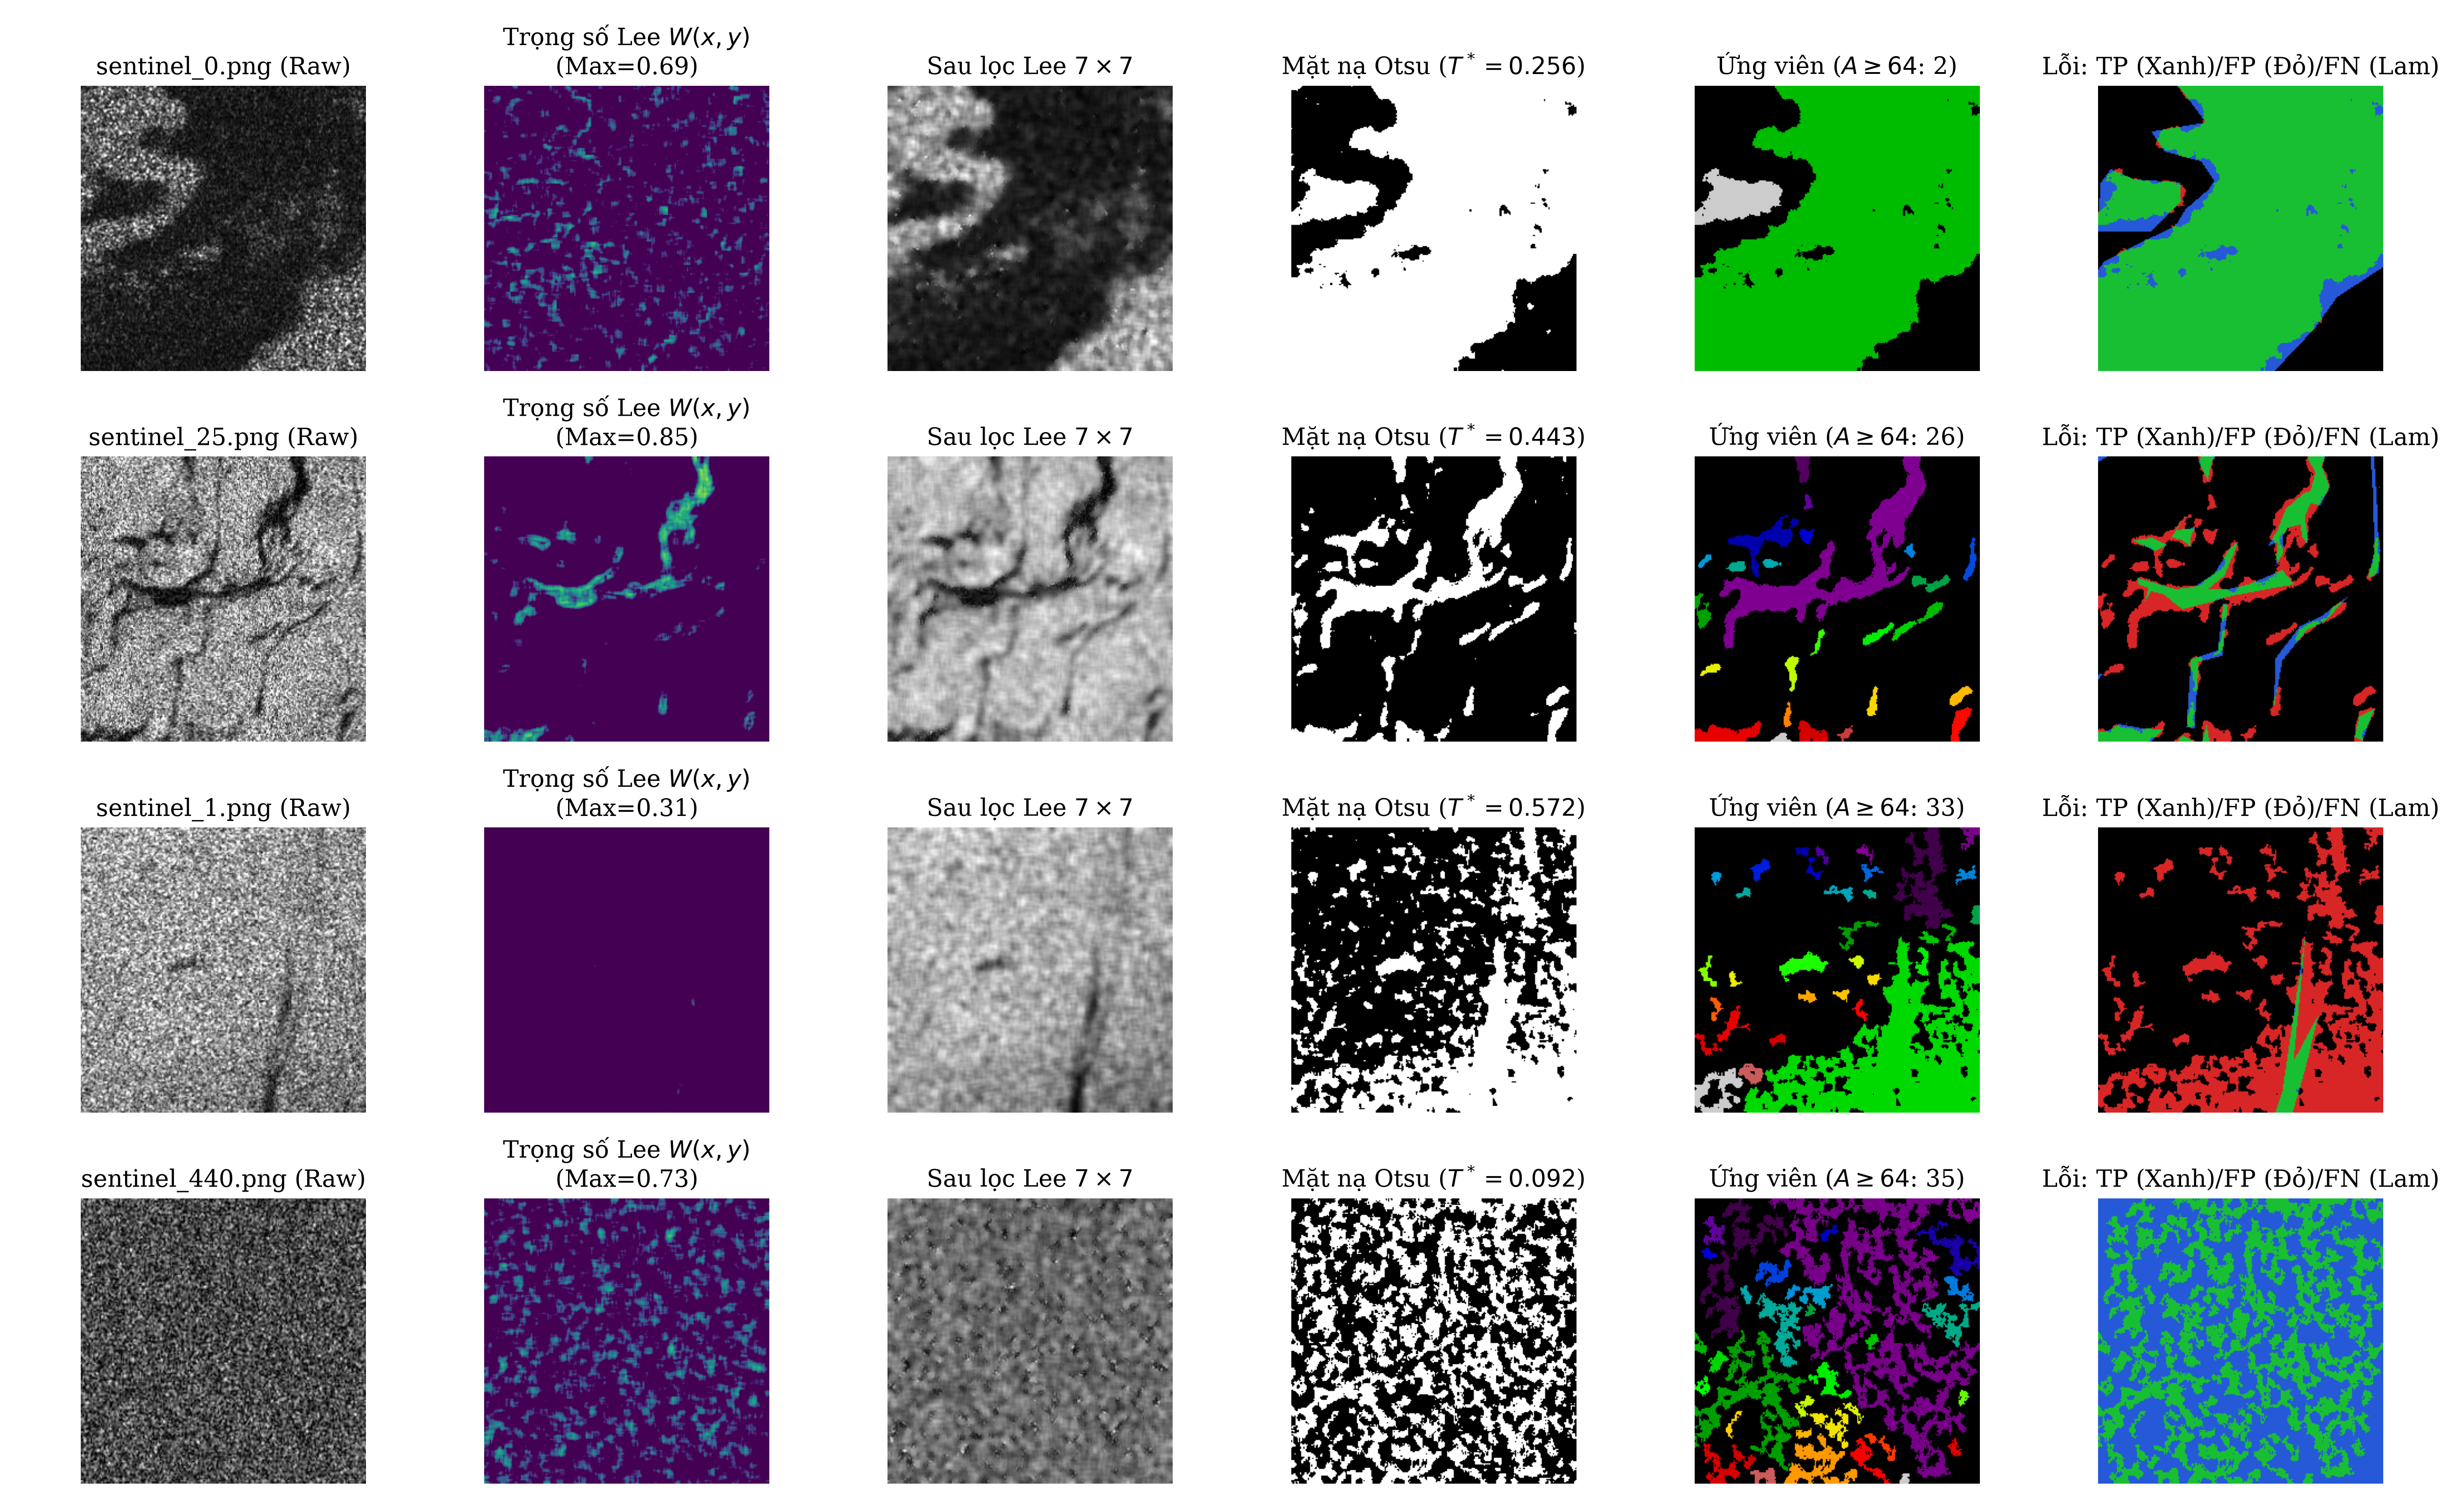
\includegraphics[width=\textwidth]{figures/fig3_step_by_step_pipeline.png}
\caption{Trực quan hóa các bước biến đổi trung gian của quy trình trên 4 cảnh SAR đại diện (\texttt{val/sentinel\_0.png}, \texttt{val/sentinel\_25.png}, \texttt{val/sentinel\_1.png}, \texttt{val/sentinel\_440.png}): Ảnh thô $\to$ Bản đồ trọng số Lee $W(x, y)$ $\to$ Ảnh sau lọc Lee $7 \times 7$ $\to$ Mặt nạ nhị phân Otsu $\to$ Vùng ứng viên sau lọc diện tích $A \ge 64$ $\to$ Bản đồ phân loại lỗi cấp điểm ảnh (True Positive: Xanh lá, False Positive: Đỏ, False Negative: Lam).}
\label{fig:step_pipeline}
\end{figure*}

\begin{table*}[!t]
\centering
\caption{So sánh có kiểm soát 13 cấu hình lọc không gian (cố định phân ngưỡng Otsu, $A_{\min} = 16$) trên toàn bộ 671 ảnh tập kiểm định (Validation). Khoảng tin cậy Bootstrap 95\% của $\Delta\text{F1}$ được tính qua $2\,000$ lần lấy mẫu lại có hoàn lại theo patch.}
\label{tab:filter_benchmark}
\resizebox{\textwidth}{!}{%
\begin{tabular}{lcccccccc}
\toprule
\textbf{Cấu hình bộ lọc} & \textbf{TP} & \textbf{FP} & \textbf{FN} & \textbf{Prec} & \textbf{Rec} & \textbf{Cand F1} & \textbf{Pix IoU} & \textbf{$\Delta\text{F1}$ vs.\ Lee $7\times 7, L=4$ (95\% CI)} \\
\midrule
\textit{None (Không lọc)} & 518 & $39\,283$ & $2\,222$ & 0.0130 & 0.1891 & 0.0244 & 0.4272 & $+0.0612 \quad [+0.0534, +0.0693]$ \\
\textit{Median $3 \times 3$} & 758 & $50\,479$ & $1\,982$ & 0.0148 & 0.2766 & 0.0281 & 0.4780 & $+0.0574 \quad [+0.0508, +0.0645]$ \\
\textit{Median $5 \times 5$} & 910 & $36\,046$ & $1\,830$ & 0.0246 & 0.3321 & 0.0458 & 0.5241 & $+0.0397 \quad [+0.0346, +0.0451]$ \\
\textit{Gaussian $\sigma = 0.8$} & 794 & $47\,039$ & $1\,946$ & 0.0166 & 0.2898 & 0.0314 & 0.4849 & $+0.0541 \quad [+0.0476, +0.0608]$ \\
\textit{Gaussian $\sigma = 1.2$} & 895 & $40\,877$ & $1\,845$ & 0.0214 & 0.3266 & 0.0402 & 0.5118 & $+0.0453 \quad [+0.0398, +0.0513]$ \\
\textit{Lee $3 \times 3$ ($L=1$)} & 821 & $46\,341$ & $1\,919$ & 0.0174 & 0.2996 & 0.0329 & 0.4909 & $+0.0526 \quad [+0.0462, +0.0592]$ \\
\textit{Lee $3 \times 3$ ($L=4$)} & 822 & $46\,897$ & $1\,918$ & 0.0172 & 0.3000 & 0.0326 & 0.4907 & $+0.0529 \quad [+0.0466, +0.0595]$ \\
\textit{Lee $5 \times 5$ ($L=1$)} & 961 & $32\,247$ & $1\,779$ & 0.0289 & 0.3507 & 0.0535 & 0.5365 & $+0.0321 \quad [+0.0278, +0.0367]$ \\
\textit{Lee $5 \times 5$ ($L=4$)} & 967 & $32\,486$ & $1\,773$ & 0.0289 & 0.3529 & 0.0534 & 0.5355 & $+0.0321 \quad [+0.0281, +0.0366]$ \\
\textit{Lee $7 \times 7$ ($L=1$)} & $1\,034$ & $20\,770$ & $1\,706$ & 0.0474 & 0.3774 & 0.0843 & 0.5645 & $+0.0013 \quad [-0.0004, +0.0031]$ \\
\textbf{Lee $7 \times 7$ ($L=4$) [Chọn]} & $\mathbf{1\,049}$ & $\mathbf{20\,743}$ & $\mathbf{1\,691}$ & \textbf{0.0481} & \textbf{0.3828} & \textbf{0.0855} & \textbf{0.5629} & \textbf{Mốc tham chiếu chuẩn} \\
\midrule
\textit{Mean $7 \times 7$ [Đối chứng]} & $1\,033$ & $20\,787$ & $1\,707$ & 0.0473 & 0.3770 & 0.0841 & 0.5646 & $+0.0014 \quad [-0.0003, +0.0033]$ \\
\textit{Median $7 \times 7$ [Đối chứng]} & 999 & $22\,856$ & $1\,741$ & 0.0419 & 0.3646 & 0.0751 & 0.5557 & $+0.0104 \quad [+0.0075, +0.0134]$ \\
\bottomrule
\end{tabular}%
}
\end{table*}

\begin{figure}[!t]
\centering
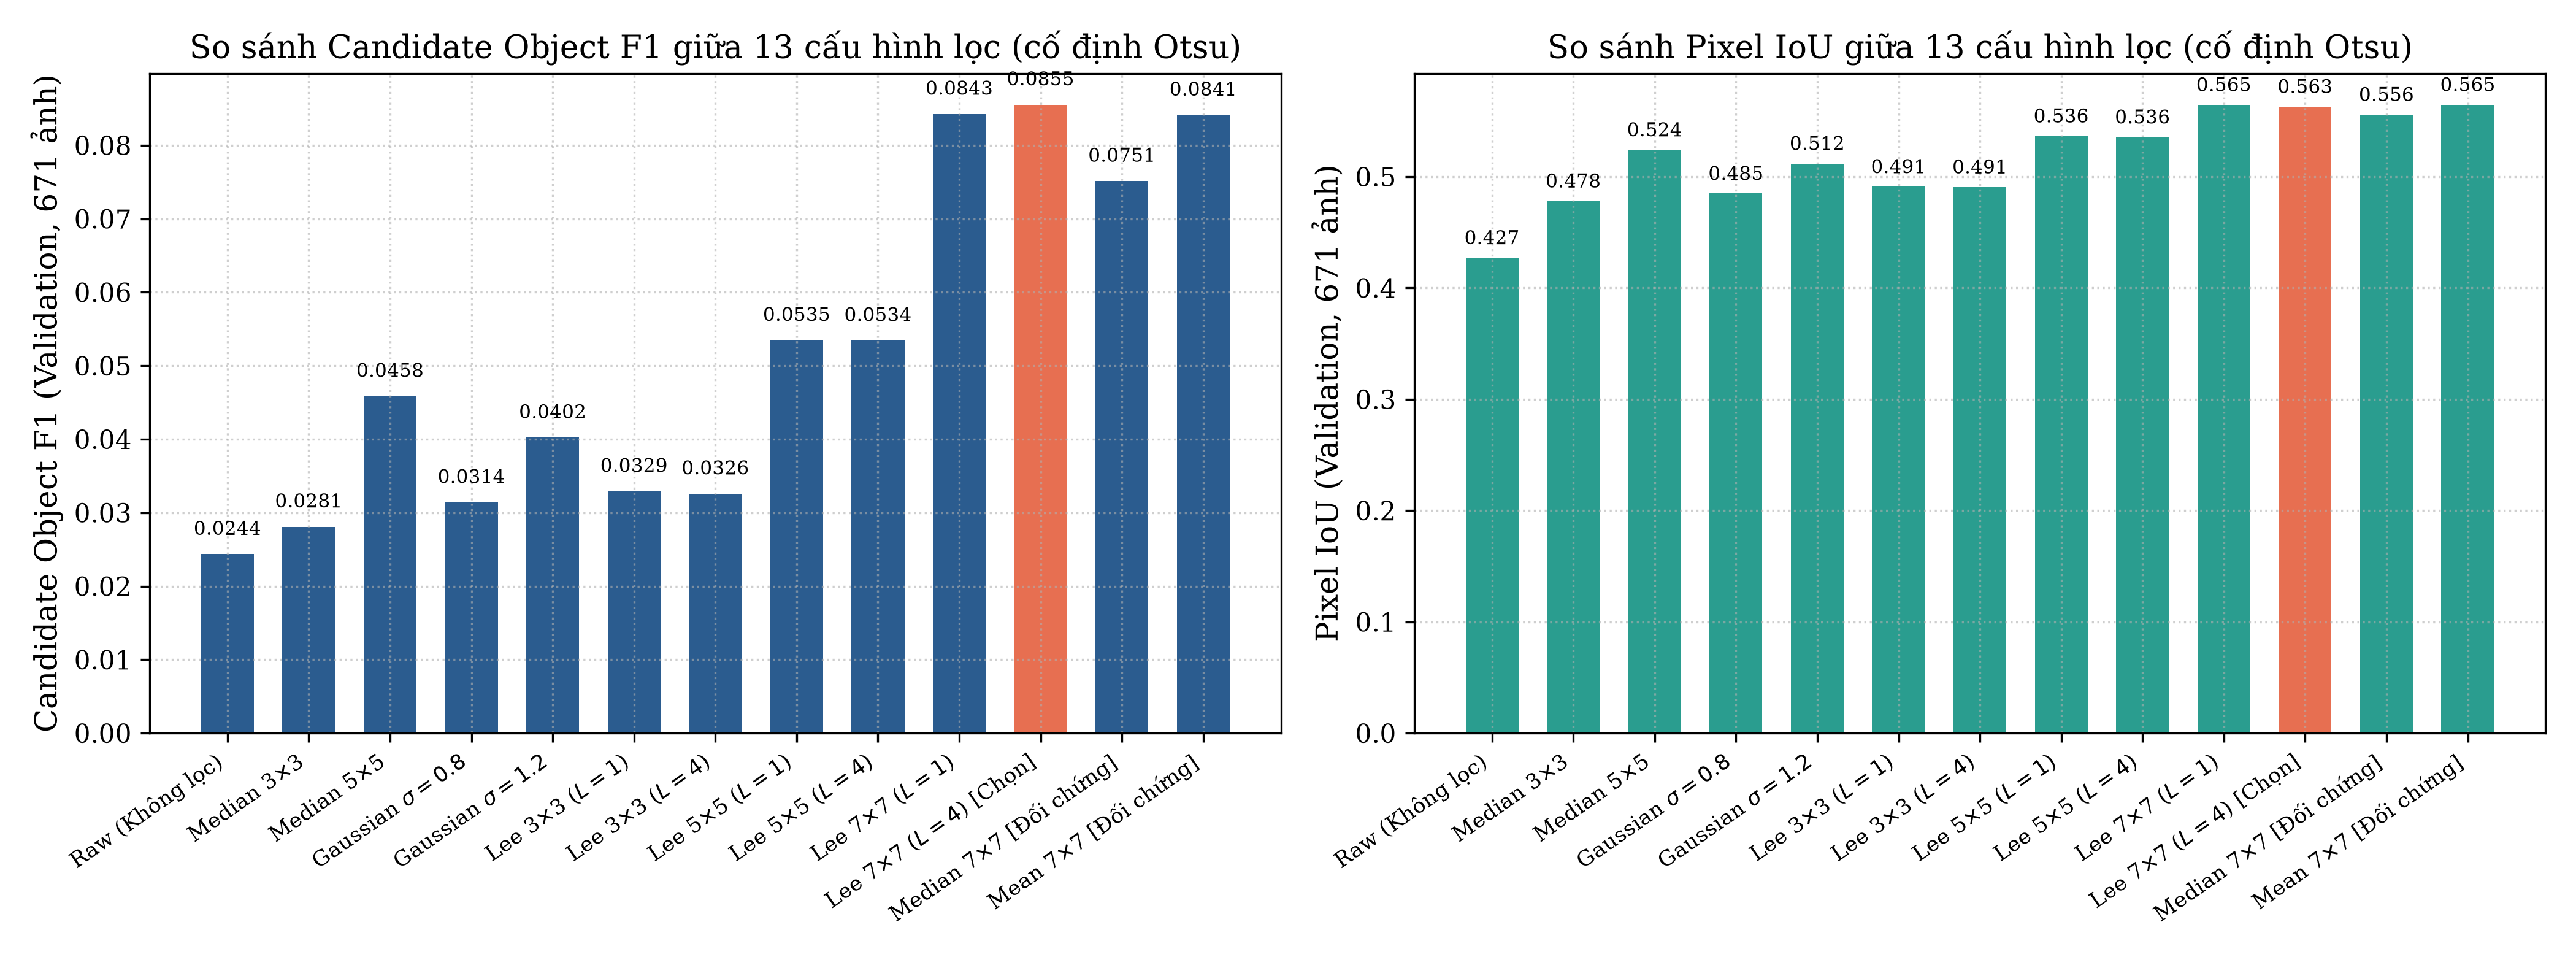
\includegraphics[width=\linewidth]{figures/fig4_filter_threshold_benchmark.png}
\caption{Đối sánh định lượng Candidate Object F1 và Pixel IoU giữa 13 cấu hình lọc không gian (cố định phân ngưỡng Otsu) trên toàn bộ 671 ảnh tập kiểm định (Validation).}
\label{fig:filter_benchmark}
\end{figure}

Kết quả thể hiện trong Bảng~\ref{tab:filter_benchmark}, Hình~\ref{fig:step_pipeline} và Hình~\ref{fig:filter_benchmark} đưa ra các phát hiện thực nghiệm quan trọng:
\begin{enumerate}
    \item \textbf{Hiệu quả giảm báo nhầm của kích thước cửa sổ lọc:} Trong lưới kích thước $\{3 \times 3, 5 \times 5, 7 \times 7\}$, việc mở rộng cửa sổ lọc lên biên trên $7 \times 7$ đóng vai trò quyết định trong việc giảm số lượng báo nhầm (từ $>46\,000$ FP xuống $\approx 20\,700$ FP, giảm hơn 55\% số mảnh nhiễu), đồng thời nâng Candidate F1 đơn điệu từ $0.0326$ ($3 \times 3$) lên $0.0534$ ($5 \times 5$) và đạt $0.0855$ ($7 \times 7$). Do $7 \times 7$ nằm tại biên trên của không gian tìm kiếm đã khóa, việc khảo sát các cửa sổ lớn hơn ($9 \times 9, 11 \times 11$) để xác định điểm uốn mà tại đó hiện tượng xóa nhòa dải dầu mảnh bắt đầu làm giảm Recall là hướng mở rộng cần thiết.
    \item \textbf{So sánh giữa Lee $7 \times 7$ và các bộ lọc đối chứng:} Trong không gian tìm kiếm ban đầu, cấu hình Lee $7 \times 7$ ($L=4$) đạt Candidate F1 cao nhất ($0.0855$). Tuy nhiên, phép đối chứng có kiểm soát bổ sung với cùng kích thước cửa sổ $7 \times 7$ cho thấy:
    \begin{itemize}
        \item Cấu hình Lee $7 \times 7$ ($L=1$, Candidate F1 $= 0.0843$) và bộ lọc trung bình Mean $7 \times 7$ (Candidate F1 $= 0.0841$) có hiệu năng tương đương thống kê với Lee $7 \times 7$ ($L=4$); độ lệch $\Delta\text{F1} = +0.0014$ so với Mean $7 \times 7$ có khoảng tin cậy Bootstrap 95\% $[-0.0003, +0.0033]$ chứa giá trị 0.
        \item Giải thích nguyên nhân: Như đã phân tích tại Mục~\ref{subsec:lee_filter}, do ảnh trong bộ dữ liệu SOS đã qua tiền xử lý đa nhìn và lượng tử hóa 8-bit ($[0, 1]$), hệ số biến thiên cục bộ $C_I^2(x, y) = v(x, y)/m^2(x, y)$ tại đại đa số các vùng biển và tâm vết dầu đều nhỏ hơn nhiều so với ngưỡng phương sai nhiễu giả định $1/L \in \{0.25, 1.0\}$. Hệ quả là $W(x, y) = \max(0, 1 - \frac{1/L}{C_I^2}) = 0$ trên toàn bộ vùng đồng nhất (như ở hàng 3 Hình~\ref{fig:step_pipeline} với $\max W = 0.00$) và chỉ kích hoạt nhẹ ($W > 0$) dọc theo ranh giới chuyển tiếp dốc. Do đó, bộ lọc Lee với $L \le 4$ trên ảnh PNG 8-bit thực chất hoạt động gần tương đương bộ lọc hộp Mean $7 \times 7$, và cả hai đều vượt trội có ý nghĩa thống kê so với Median $7 \times 7$ ($\Delta\text{F1} = +0.0104$, 95\% CI $[+0.0075, +0.0134]$).
    \end{itemize}
    \item \textbf{Nhánh phân ngưỡng cục bộ Niblack:} Khảo sát đầy đủ 9 cấu hình Niblack (kết hợp cùng bộ lọc Lee $7 \times 7, L=4$ tại $A_{\min} = 16$) trên tập kiểm định cho thấy hiệu năng suy giảm mạnh do hiện tượng bùng nổ báo nhầm ở vùng biển đồng nhất:
    \begin{itemize}
        \item Cửa sổ $15 \times 15$: $k=0.2 \to \text{F1}=0.0067$ ($\text{TP}=255, \text{FP}=75\,870$); $k=0.5 \to \text{F1}=0.0031$ ($\text{FP}=139\,556$); $k=0.8 \to \text{F1}=0.0013$ ($\text{FP}=154\,728$).
        \item Cửa sổ $31 \times 31$: $k=0.2 \to \text{F1}=0.0232$ ($\text{TP}=561, \text{FP}=46\,595$); $k=0.5 \to \text{F1}=0.0134$ ($\text{FP}=76\,925$); $k=0.8 \to \text{F1}=0.0083$ ($\text{FP}=89\,203$).
        \item Cửa sổ $51 \times 51$: $k=0.2 \to \text{F1}=0.0319$ ($\text{TP}=696, \text{FP}=40\,268, \text{IoU}=0.3144$); $k=0.5 \to \text{F1}=0.0241$ ($\text{FP}=59\,676$); $k=0.8 \to \text{F1}=0.0178$ ($\text{FP}=66\,610$).
    \end{itemize}
    Ngay cả cấu hình Niblack tốt nhất trên toàn bộ lưới 110 cấu hình (Lee $7 \times 7, L=1$ + Niblack $51 \times 51, k=0.2$) cũng chỉ đạt Candidate F1 $= 0.0325$, và sau khi ghép bộ phân loại học máy trên tập kiểm định chỉ đạt F1 $= 0.1447$ (CART) và $0.1380$ (LinearSVM). Ngưỡng cục bộ $T(x, y) = m_W - k s_W$ bị hạ thấp ở các vùng biển lặng gió tạo ra hàng chục nghìn mảnh tối vụn, do đó phân ngưỡng toàn cục Otsu là lựa chọn phù hợp hơn cho bước tạo ứng viên trên bộ dữ liệu này.
\end{enumerate}

\subsection{Phân tích đặc trưng, Khảo sát Ablation và Quá trình hội tụ SVM}
\label{subsec:feature_analysis}

\begin{figure*}[!t]
\centering
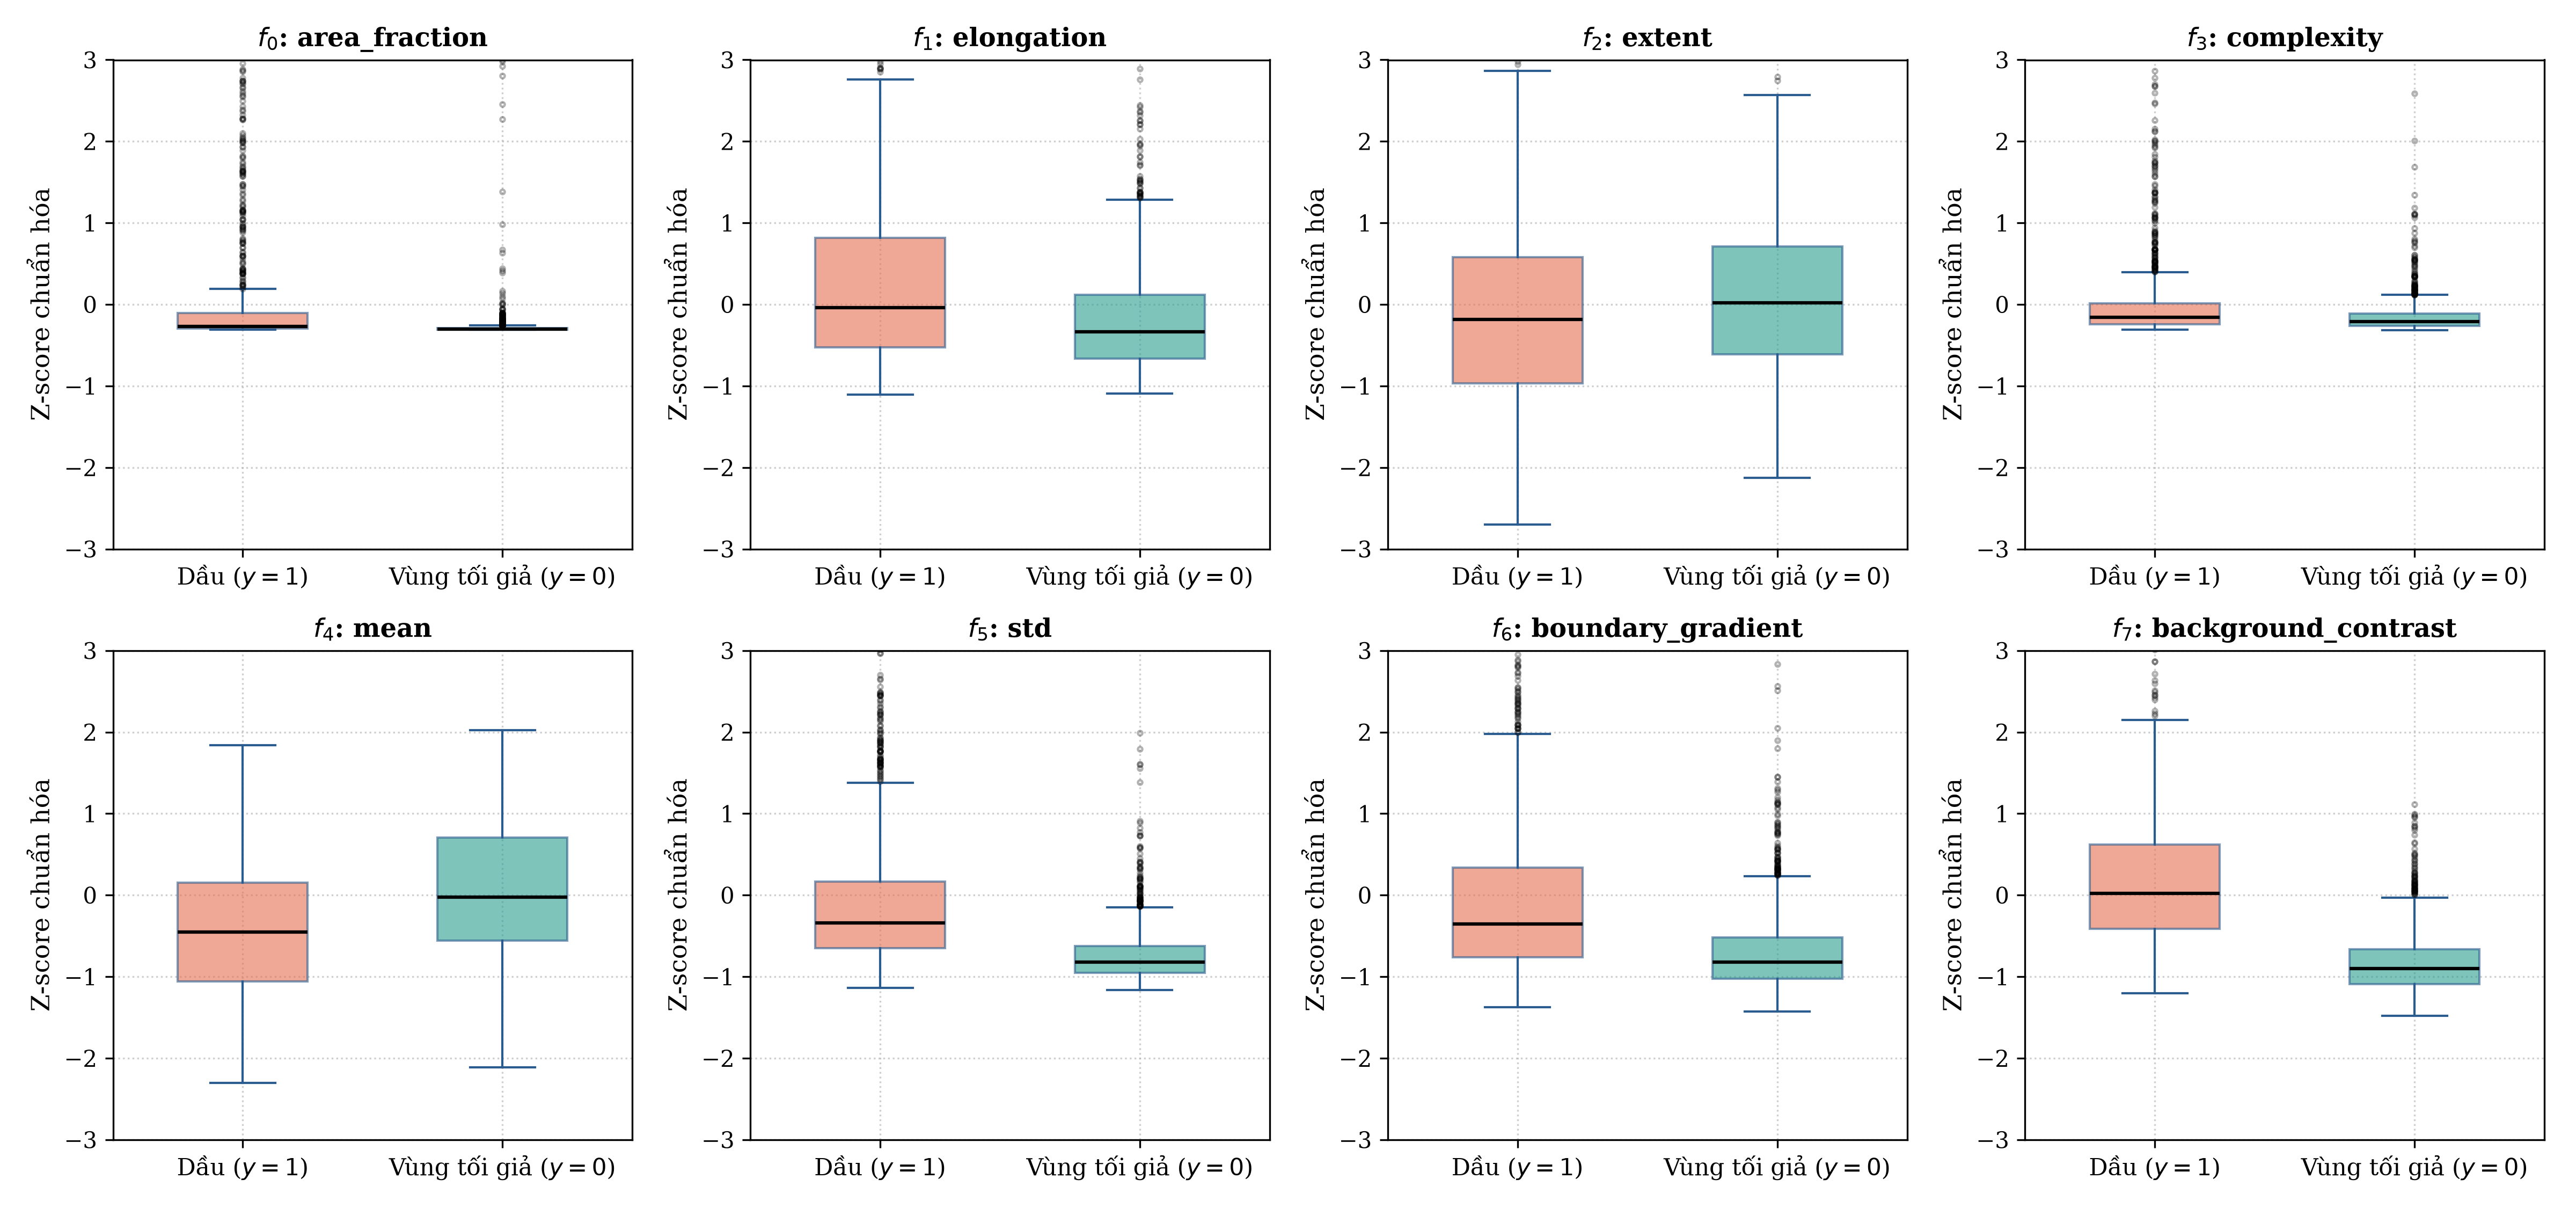
\includegraphics[width=0.95\textwidth]{figures/fig5_feature_distributions.png}
\caption{Biểu đồ Boxplot so sánh phân bố Z-score chuẩn hóa của 8 đặc trưng vùng giữa lớp Vết dầu thật ($\mathrm{Purity} \ge 0.50$, màu cam) và lớp Vùng tối báo nhầm ($\mathrm{Purity} \le 0.05$, màu xanh ngọc).}
\label{fig:feature_distributions}
\end{figure*}

\begin{figure}[!t]
\centering
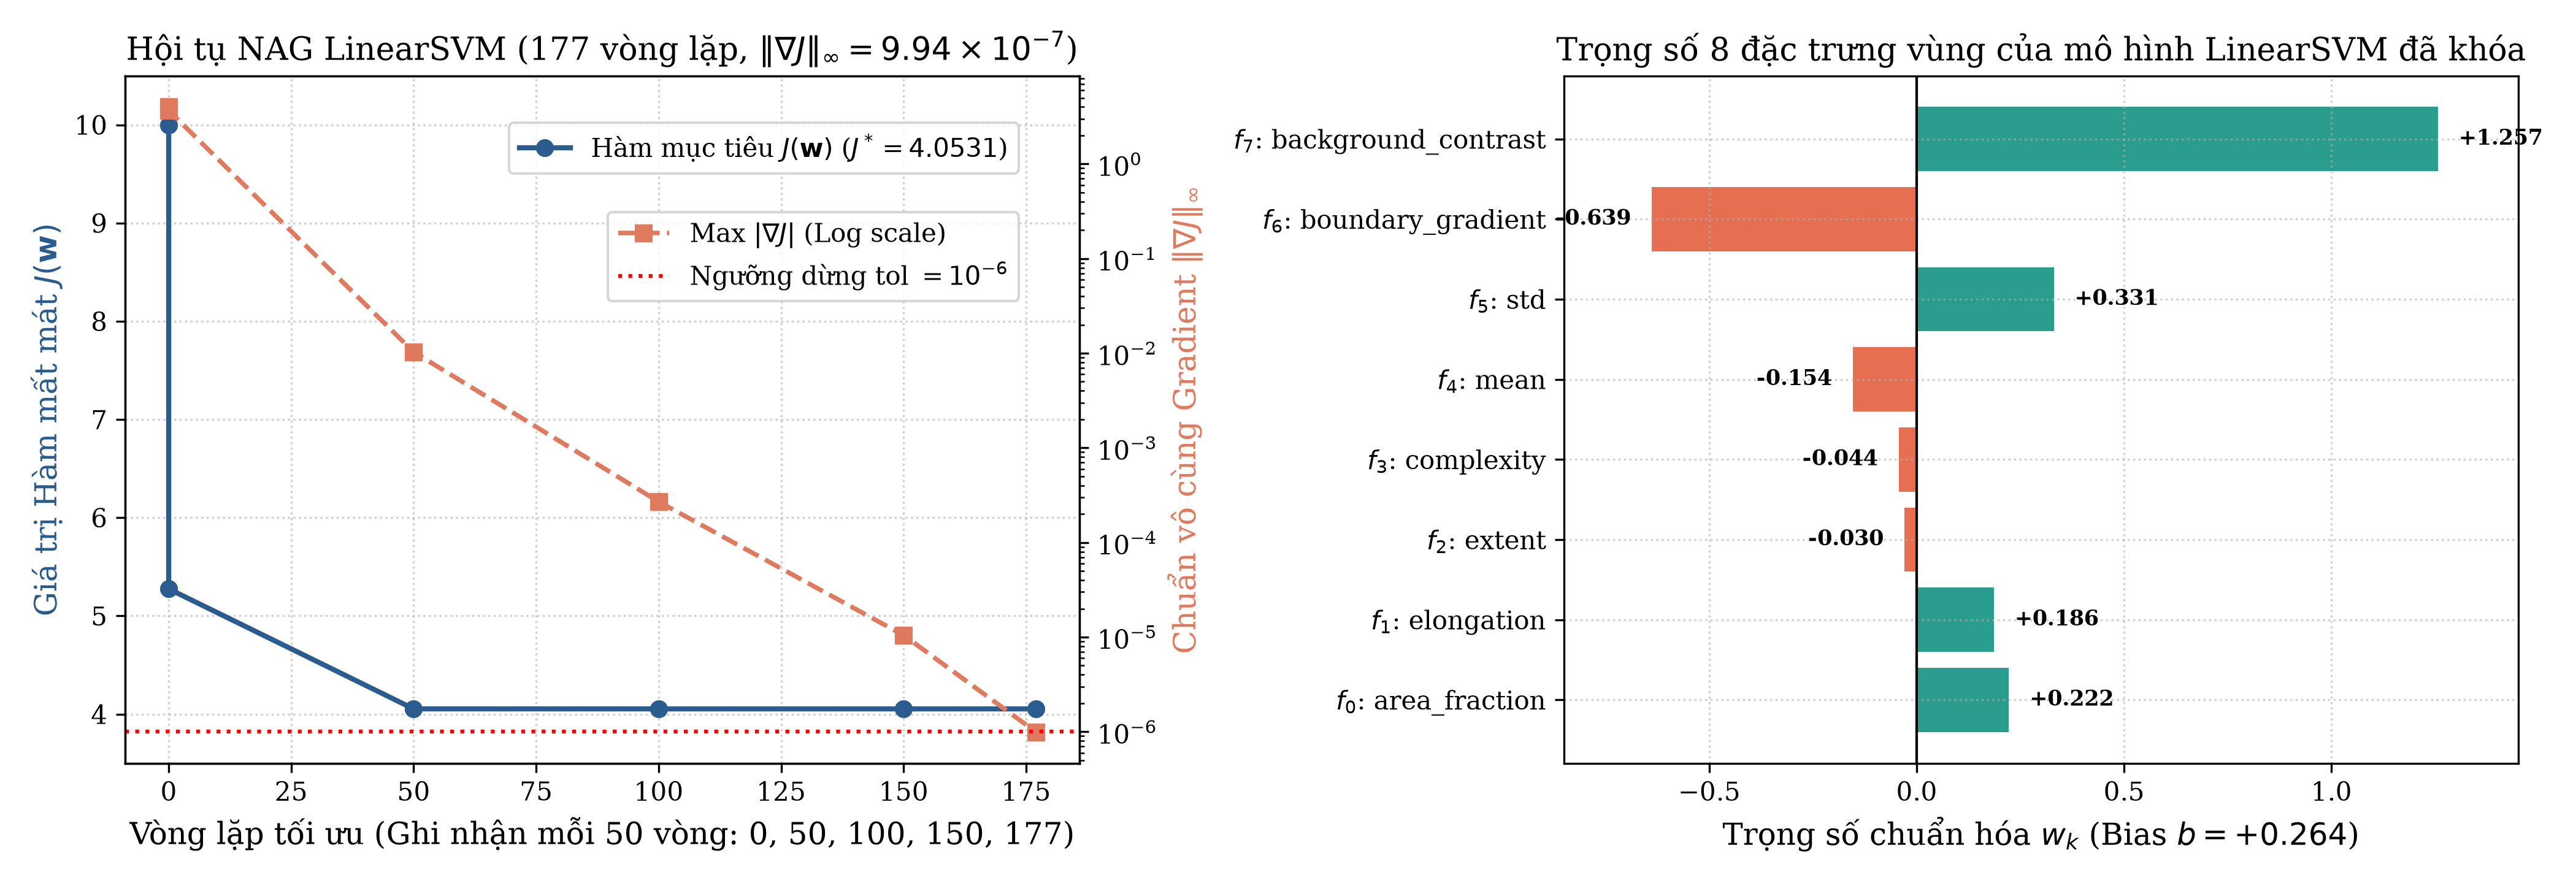
\includegraphics[width=\linewidth]{figures/fig6_svm_convergence_weights.png}
\caption{Đường cong hội tụ của thuật toán NAG ghi nhận tại các mốc 50 vòng lặp ($0, 50, 100, 150, 177$) cùng biểu đồ trọng số chuẩn hóa $w_k$ của 8 đặc trưng vùng trong mô hình LinearSVM đã khóa.}
\label{fig:svm_convergence}
\end{figure}

\begin{table}[!t]
\centering
\caption{Khảo sát hậu xử lý hình thái học, loại bỏ nhóm đặc trưng (Ablation study) và đối sánh mô hình trên tập kiểm định (671 ảnh Validation Sentinel-1A).}
\label{tab:ablation_validation}
\resizebox{\linewidth}{!}{%
\begin{tabular}{lccccc}
\toprule
\textbf{Cấu hình khảo sát} & \textbf{TP} & \textbf{FP} & \textbf{FN} & \textbf{Object F1} & \textbf{Pixel IoU} \\
\midrule
\multicolumn{6}{l}{\textit{Khảo sát ngưỡng diện tích $A_{\min}$ và hình thái học (Lee $7\times 7, L=4$ + Otsu + SVM):}} \\
$A_{\min} = 4$, \texttt{none} (Không đóng/mở) & $1\,035$ & $8\,571$ & $1\,705$ & 0.1677 & 0.6267 \\
$A_{\min} = 16$, \texttt{none} (Không đóng/mở) & $1\,034$ & $4\,482$ & $1\,706$ & 0.2505 & 0.6376 \\
$A_{\min} = 64$, \texttt{none} (\textbf{Chọn theo quy tắc}) & $\mathbf{1\,016}$ & $2\,215$ & $\mathbf{1\,724}$ & 0.3403 & \textbf{0.6524} \\
$A_{\min} = 64$, \texttt{close} (Đóng hình thái $3\times 3$) & 971 & $\mathbf{1\,961}$ & $1\,769$ & \textbf{0.3424} & 0.6402 \\
$A_{\min} = 64$, \texttt{open\_close} (Mở--Đóng $3\times 3$) & 988 & $2\,230$ & $1\,752$ & 0.3317 & 0.6505 \\
\midrule
\multicolumn{6}{l}{\textit{Ablation theo nhóm đặc trưng (LinearSVM, $C=10, A_{\min}=64$, \texttt{none}):}} \\
Chỉ đặc trưng hình học (\texttt{shape}, 4 chiều) & 736 & $1\,737$ & $2\,004$ & 0.2824 & 0.5899 \\
Chỉ đặc trưng bức xạ/biên (\texttt{intensity}, 4 chiều) & $1\,002$ & $2\,188$ & $1\,738$ & 0.3379 & \textbf{0.6542} \\
Kết hợp toàn bộ 8 đặc trưng (\texttt{all}, đề xuất) & $\mathbf{1\,016}$ & $2\,215$ & $\mathbf{1\,724}$ & \textbf{0.3403} & 0.6524 \\
\midrule
\multicolumn{6}{l}{\textit{So sánh bộ phân loại (Nhóm đặc trưng \texttt{all}, $A_{\min}=64$, \texttt{none}):}} \\
Cây quyết định CART ($\text{depth}=3, \text{leaf}=20$) & 961 & $\mathbf{1\,998}$ & $1\,779$ & 0.3373 & 0.6456 \\
LinearSVM ($C=10$, đề xuất) & $\mathbf{1\,016}$ & $2\,215$ & $\mathbf{1\,724}$ & \textbf{0.3403} & \textbf{0.6524} \\
\midrule
\multicolumn{6}{l}{\textit{Đánh giá cấp độ ứng viên theo nhãn Purity ($\mathrm{Purity} \ge 0.50$ vs.\ $\le 0.05$, $9\,287$ mẫu Val):}} \\
CART ($\text{TN}=6\,008$, Prec $=0.7952$, Rec $=0.7722$) & $2\,112$ & 544 & 623 & 0.7835 & -- \\
LinearSVM ($\text{TN}=5\,940$, Prec $=0.7874$, Rec $=0.8285$) & $\mathbf{2\,266}$ & 612 & $\mathbf{469}$ & \textbf{0.8074} & -- \\
\midrule
\multicolumn{6}{l}{\textit{Độ nhạy theo ngưỡng nhị phân Ground Truth (LinearSVM):}} \\
Ngưỡng mặt nạ GT $M_{\text{raw}} \ge 64$ & $1\,027$ & $2\,204$ & $1\,690$ & 0.3453 & 0.6526 \\
Ngưỡng mặt nạ GT $M_{\text{raw}} \ge 128$ (Chuẩn) & $1\,016$ & $2\,215$ & $1\,724$ & 0.3403 & 0.6524 \\
Ngưỡng mặt nạ GT $M_{\text{raw}} \ge 192$ & $1\,010$ & $2\,221$ & $1\,752$ & 0.3371 & 0.6517 \\
\bottomrule
\end{tabular}%
}
\end{table}

Hình~\ref{fig:feature_distributions} biểu diễn phân bố Z-score của 8 đặc trưng vùng giữa hai lớp, và Hình~\ref{fig:svm_convergence} thể hiện đường cong hội tụ cùng trọng số của mô hình LinearSVM đã khóa. Các kết quả mang lại các quan sát định lượng rõ ràng:
\begin{itemize}
    \item \textbf{Trọng số và cơ chế phân loại của LinearSVM:} Trong vector trọng số chuẩn hóa 9 chiều ($\mathbf{w} \in \mathbb{R}^8$ và hệ số chặn $b = +0.264$), trọng số dương lớn nhất thuộc về \texttt{background\_contrast} ($w_7 = +1.257$), theo sau bởi \texttt{std} ($w_5 = +0.331$), \texttt{area\_fraction} ($w_0 = +0.222$) và \texttt{elongation} ($w_1 = +0.186$). Ngược lại, trọng số âm lớn nhất rơi vào \texttt{boundary\_gradient} ($w_6 = -0.639$) và \texttt{mean} ($w_4 = -0.154$), trong khi \texttt{complexity} ($w_3 = -0.044$) và \texttt{extent} ($w_2 = -0.030$) nhận trọng số âm nhỏ.
    \item \textbf{Giải thích hiện tượng đa cộng tuyến và biến ức chế (Suppressor Variable) tại $w_6 = -0.639$:} Quan sát Hình~\ref{fig:feature_distributions} cho thấy xét đơn biến (univariate), các vùng dầu thật ($y=1$) thực tế có trung vị \texttt{boundary\_gradient} ($f_6$) cao hơn vùng tối giả ($y=0$), với hệ số tương quan điểm--nhị phân dương $\mathrm{Corr}(f_6, y) = +0.3632$ (cùng chiều với $\mathrm{Corr}(f_7, y) = +0.6485$, $\mathrm{Corr}(f_5, y) = +0.4499$ và ngược chiều với $\mathrm{Corr}(f_4, y) = -0.3413$). Tuy nhiên, trong mô hình tuyến tính đa biến, $f_6$ lại mang trọng số âm lớn $w_6 = -0.639$. Phân tích ma trận tương quan trên tập huấn luyện làm sáng tỏ nguyên nhân: \texttt{boundary\_gradient} có tương quan dương rất mạnh với cả độ lệch chuẩn nội vùng $\mathrm{Corr}(f_6, f_5) = +0.8504$ lẫn độ tương phản nền $\mathrm{Corr}(f_6, f_7) = +0.6716$. Khi tổ hợp tuyến tính đã gán trọng số dương rất lớn cho $w_7 = +1.257$ và $w_5 = +0.331$, đặc trưng $f_6$ đóng vai trò là một \textit{biến ức chế (suppressor variable)} cổ điển: trọng số âm $w_6 = -0.639$ giúp hiệu chỉnh phần phương sai dư thừa của các vùng có đạo hàm biên gắt nhân tạo do cắt ngưỡng hoặc nhiễu cục bộ ($f_6$ lớn, $f_5$ lớn) nhưng không đi kèm độ chênh lệch tương phản nền tương xứng ($f_7$).
    \item \textbf{Khảo sát hình thái học, ngưỡng diện tích và Ablation (Bảng~\ref{tab:ablation_validation}):}
    \begin{enumerate}
        \item \textit{Tác động của $A_{\min}$ và phép đóng/mở hình thái:} Việc nâng ngưỡng diện tích tối thiểu từ $A_{\min} = 4$ lên $16$ và $64$ pixels giúp cắt giảm mạnh số lượng mảnh nhiễu (từ $8\,571$ xuống $4\,482$ và $2\,215$ FP) trong khi hầu như không làm giảm số lượng đối tượng đúng ($\text{TP}$ chỉ giảm nhẹ từ $1\,035$ xuống $1\,016$), qua đó nâng Object F1 từ $0.1677$ lên $0.3403$. Tại mức $A_{\min} = 64$, phép đóng hình thái \texttt{close} đạt Object F1 cao hơn nhẹ ($0.3424$ so với $0.3403$ của \texttt{none}), nhưng vì chênh lệch này nằm trong dải dung sai lựa chọn $\Delta\text{F1} \le 0.005$ đã định nghĩa trước ở Mục~\ref{subsec:dataset}, quy tắc ưu tiên độ thu hồi Recall cao hơn ($0.3708$ với $1\,016$ TP của \texttt{none} so với $0.3544$ với $971$ TP của \texttt{close}) đã chọn cấu hình \texttt{none} để tránh làm dính liền các vệt dầu lân cận.
        \item \textit{Đóng góp của các nhóm đặc trưng:} Nhóm đặc trưng bức xạ/biên (\texttt{intensity}, 4 chiều) giữ vai trò quyết định với Object F1 $= 0.3379$ và Pixel IoU $= 0.6542$, vượt xa nhóm đặc trưng hình học thuần túy (\texttt{shape}, F1 $= 0.2824$). Việc bổ sung 4 đặc trưng hình học vào nhóm bức xạ (\texttt{all}, 8 chiều) mang lại mức cải thiện khiêm tốn ($+0.0024$ Object F1, từ $0.3379$ lên $0.3403$), khẳng định thông tin bức xạ đóng vai trò chủ đạo trên bộ dữ liệu này.
        \item \textit{So sánh LinearSVM và CART:} Trên thước đo đối tượng Hungarian ($\IoU \ge 0.50$), hai mô hình có hiệu năng sát nhau (LinearSVM đạt F1 $= 0.3403$, Recall $= 0.3708$; CART đạt F1 $= 0.3373$, Precision cao hơn ở mức $0.3248$). Xét riêng ở cấp độ phân loại từng ứng viên theo nhãn Purity ($\mathrm{Purity} \ge 0.50$ so với $\le 0.05$ trên $9\,287$ mẫu kiểm định rõ nghĩa), LinearSVM đạt F1 cấp ứng viên $80.74\%$ ($\text{TP}=2\,266, \text{FP}=612, \text{TN}=5\,940, \text{FN}=469$), nhỉnh hơn CART ($78.35\%$, $\text{TP}=2\,112, \text{FP}=544, \text{TN}=6\,008, \text{FN}=623$) nhờ giữ lại nhiều hơn $154$ vùng dầu thật. Cả hai bản tự cài bằng NumPy đều đạt độ đồng thuận dự đoán 100\% so với triển khai tham chiếu \texttt{scikit-learn}.
    \end{enumerate}
    \item \textbf{Quá trình hội tụ NAG:} Thuật toán NAG hội tụ sau 177 vòng lặp (Hình~\ref{fig:svm_convergence} vẽ theo chu kỳ ghi nhật ký mỗi 50 vòng lặp tại các mốc $0, 50, 100, 150$ và điểm dừng $177$), đưa hàm mục tiêu từ $J(\mathbf{0}) = 10.0$ xuống $J^* = 4.0531$ và đạt chuẩn vô cùng gradient $\|\nabla J\|_\infty = 9.94 \times 10^{-7} \le 10^{-6}$.
\end{itemize}

\subsection{Đánh giá so sánh định lượng và định tính trên tập kiểm thử độc lập}
\label{subsec:quantitative_eval}

\begin{table*}[!t]
\centering
\caption{Đánh giá so sánh hiệu năng trên tập kiểm thử độc lập (839 ảnh Sentinel-1A và 776 ảnh ALOS PALSAR). Giao thức ghép cặp đối tượng Hungarian ở ngưỡng $\IoU \ge 0.5$. Khoảng tin cậy Bootstrap 95\% trên tập Sentinel-1A: Object F1 đạt $0.2805 \ [0.2652, 0.2980]$ (LinearSVM) so với $0.1220 \ [0.1124, 0.1328]$ (Không Classifier), mức tăng $\Delta\text{F1} = +0.1586 \ [+0.1474, +0.1706]$.}
\label{tab:model_comparison}
\resizebox{\textwidth}{!}{%
\begin{tabular}{lcccccccccc}
\toprule
\textbf{Phương pháp} & \textbf{Ảnh} & \textbf{TP} & \textbf{FP} & \textbf{FN} & \textbf{Prec} & \textbf{Rec} & \textbf{Obj F1} & \textbf{Pix IoU} & \textbf{FP/ảnh} & \textbf{Edge / Int Rec} \\
\midrule
\textit{Baseline (Ảnh thô + Otsu, $A_{\min} = 16$)} & 839 & 426 & $49\,182$ & $2\,756$ & 0.0086 & 0.1339 & 0.0161 & 0.4367 & 58.62 & 0.1979 / 0.0038 \\
\textit{Lee 7$\times$7 + Otsu ($A_{\min} = 64$, Không Clf)} & 839 & $1\,018$ & $12\,495$ & $2\,164$ & 0.0753 & \textbf{0.3199} & 0.1220 & 0.5867 & 14.89 & \textbf{0.4221} / \textbf{0.1124} \\
\textbf{Pipeline + LinearSVM ($A_{\min} = 64$, Đề xuất)} & 839 & 996 & $\mathbf{2\,923}$ & $2\,186$ & \textbf{0.2541} & 0.3130 & \textbf{0.2805} & \textbf{0.6614} & \textbf{3.48} & 0.4156 / 0.1048 \\
\quad \textit{Macro từng ảnh ($\text{mean} \pm \text{SD}$)$^{\dagger}$} & \multicolumn{4}{c}{--} & $0.356 \pm 0.336$ & $0.446 \pm 0.382$ & $0.349 \pm 0.317$ & $0.577 \pm 0.261$ & $3.48 \pm 3.97$ & -- \\
\midrule
\textit{Ngoài cảm biến: PALSAR (LinearSVM, $A_{\min} = 64$)} & 776 & $1\,441$ & $2\,305$ & $2\,553$ & 0.3847 & 0.3608 & 0.3724 & 0.6423 & 2.97 & 0.4587 / 0.1890 \\
\quad \textit{Macro từng ảnh ($\text{mean} \pm \text{SD}$)$^{\ddagger}$} & \multicolumn{4}{c}{--} & $0.465 \pm 0.342$ & $0.438 \pm 0.338$ & $0.412 \pm 0.312$ & $0.579 \pm 0.234$ & $2.97 \pm 3.43$ & -- \\
\bottomrule
\multicolumn{11}{l}{\footnotesize $^{\dagger}$Cỡ mẫu mẫu số khác không trên Sentinel-1A (839 ảnh): $n_{\text{Prec}}=786$, $n_{\text{Rec}}=808$, $n_{\text{F1}}=n_{\text{IoU}}=814$ ($25$ ảnh $R_0$ có $\text{TP}=\text{FP}=\text{FN}=0$).} \\
\multicolumn{11}{l}{\footnotesize $^{\ddagger}$Cỡ mẫu mẫu số khác không trên ALOS PALSAR (776 ảnh): $n_{\text{Prec}}=705$, $n_{\text{Rec}}=731$, $n_{\text{F1}}=n_{\text{IoU}}=734$ ($42$ ảnh $R_0$ có $\text{TP}=\text{FP}=\text{FN}=0$).}
\end{tabular}%
}
\end{table*}

\begin{figure*}[!t]
\centering
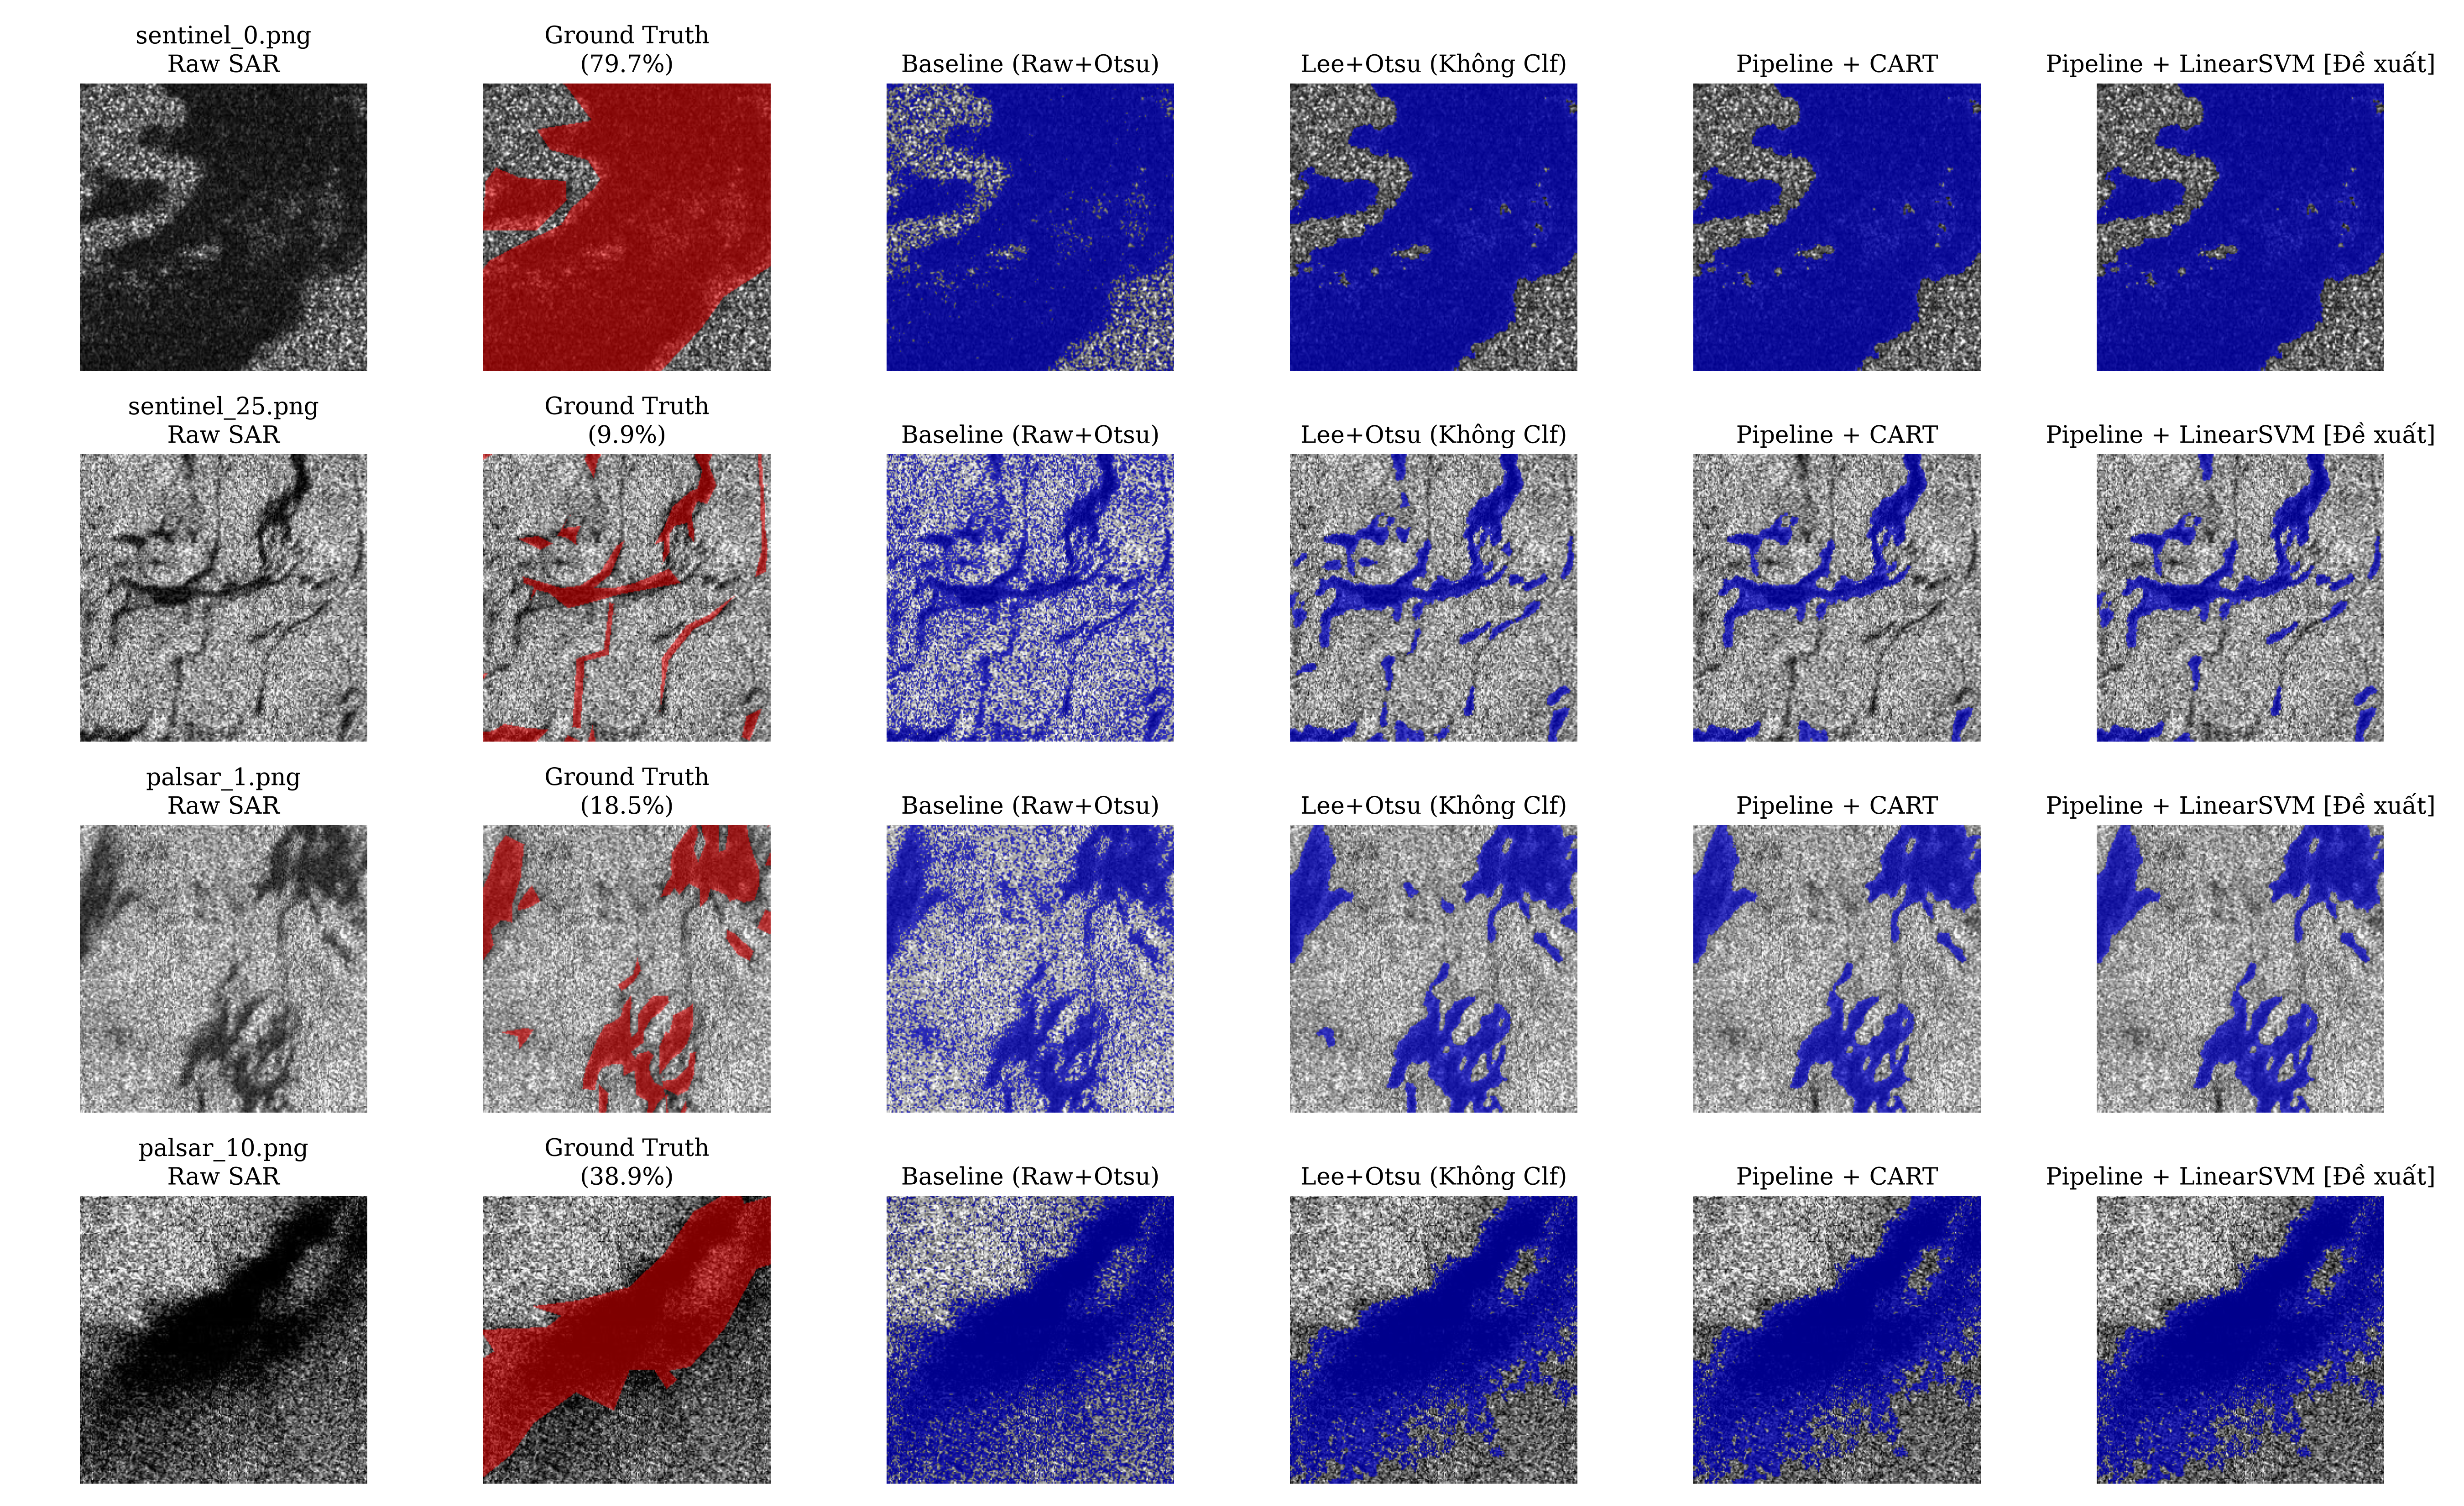
\includegraphics[width=\textwidth]{figures/fig7_qualitative_comparison.png}
\caption{Đối sánh định tính kết quả phân đoạn giữa các mô hình trên 4 cảnh SAR điển hình (\texttt{val/sentinel\_0.png}, \texttt{val/sentinel\_25.png}, \texttt{val/palsar\_1.png}, \texttt{val/palsar\_10.png}): Cột 1: Ảnh thô; Cột 2: Mặt nạ Ground Truth; Cột 3: Baseline (Ảnh thô + Otsu, $A_{\min}=16$); Cột 4: Lọc Lee + Otsu ($A_{\min}=64$, Không classifier); Cột 5: Pipeline + CART; Cột 6: Pipeline + LinearSVM (Đề xuất).}
\label{fig:qualitative_comparison}
\end{figure*}

Bảng~\ref{tab:model_comparison} tổng hợp kết quả đánh giá thực nghiệm định lượng trên tập kiểm thử độc lập ($839$ ảnh Sentinel-1A, chứa tổng cộng $3\,182$ đối tượng dầu Ground Truth). Các số liệu thực nghiệm làm rõ đóng góp của từng thành phần cũng như các giới hạn cấu trúc của phương pháp:
\begin{itemize}
    \item \textbf{Bóc tách hiệu quả của Giai đoạn 1 và Giai đoạn 2:}
    \begin{enumerate}
        \item \textit{Từ Baseline thô sang Giai đoạn 1 (Lọc Lee $7 \times 7$ + Otsu + $A_{\min} = 64$):} Tỷ lệ báo nhầm giảm từ $58.62$ xuống $14.89$ FP/ảnh (tổng số ứng viên giảm từ $49\,608$ xuống $13\,513$), đồng thời số đối tượng dầu phát hiện đúng tăng từ $426$ lên $1\,018$ TP. Lưu ý rằng bước nhảy này là kết quả tổng hợp của hai yếu tố: bộ lọc Lee $7 \times 7$ làm mượt nhiễu đốm (giúp giảm $\approx 47\%$ số FP ở cùng ngưỡng $A_{\min} = 16$, như đã chứng minh có kiểm soát tại Bảng~\ref{tab:filter_benchmark}) và việc nâng ngưỡng cắt tỉa diện tích từ $A_{\min} = 16$ (của Baseline mặc định) lên $A_{\min} = 64$ (giúp loại bỏ tiếp hơn một nửa số mảnh nhiễu nhỏ còn lại, như đã bóc tách tại Bảng~\ref{tab:ablation_validation}).
        \item \textit{Từ Giai đoạn 1 sang Giai đoạn 2 (Bổ sung bộ phân loại LinearSVM ở cùng $A_{\min} = 64$):} Đây là phép so sánh có kiểm soát hoàn toàn cho riêng bộ phân loại vùng. So với cấu hình \textit{Không dùng Classifier} ($\text{TP}=1\,018, \text{FP}=12\,495$), LinearSVM đã \textbf{loại bỏ được $9\,572$ vùng báo nhầm} (giảm $76.6\%$ FP/ảnh, từ $14.89$ xuống $3.48$ FP/ảnh), trong khi \textbf{giữ lại được $97.8\%$ số đối tượng đúng của giai đoạn tạo ứng viên} ($996 / 1\,018$ TP, chỉ mất 22 vùng và đạt độ thu hồi tổng thể $\text{Recall} = 0.3130$ trên tổng số $3\,182$ đối tượng GT toàn tập). Nhờ đó, Precision tăng $3.37$ lần (từ $0.0753$ lên $0.2541$), Object F1 tăng từ $0.1220$ lên $0.2805$ ($\Delta\text{F1} = +0.1586$, 95\% CI $[+0.1474, +0.1706]$) và Pixel IoU toàn cục tăng từ $0.5867$ lên $0.6614$.
    \end{enumerate}
    \item \textbf{Giải phẫu sự vênh giữa độ chính xác phân loại Purity và chỉ số Object F1:} Một câu hỏi quan trọng là vì sao LinearSVM đạt F1 cấp độ ứng viên tới $80.74\%$ theo nhãn Purity nhưng Object F1 cuối cùng chỉ đạt $0.3403$ (Validation) và $0.2805$ (Test). Đối chiếu ma trận nhầm lẫn cấp ứng viên trên tập Validation (Bảng~\ref{tab:ablation_validation}) với kết quả ghép cặp Hungarian ($\text{TP}_{\text{IoU}} = 1\,016, \text{FP}_{\text{IoU}} = 2\,215$) cho thấy: trong số $2\,878$ vùng được LinearSVM dự đoán là dầu ($\hat{y}_i = 1$ trên các mẫu rõ nghĩa), chỉ có \textbf{$612$ vùng ($21.3\%$) là báo nhầm nền biển thực sự} ($\mathrm{Purity} \le 0.05$). Ngược lại, có tới \textbf{$2\,266$ vùng dự đoán dương tính thực sự nằm đè lên vết dầu thật} ($\mathrm{Purity} \ge 0.50$), nhưng chỉ có $1\,016$ vùng trong số đó vượt qua ngưỡng ghép cặp 1--1 $\IoU \ge 0.50$ để trở thành $\text{TP}_{\text{IoU}}$; hơn \textbf{$1\,250$ mảnh dầu thật còn lại bị giao thức Hungarian xếp vào nhóm $\text{FP}_{\text{IoU}}$} (chiếm tới $56.4\%$ tổng số $2\,215$ FP đối tượng!). Nói cách khác, phần lớn ``False Positives'' ở cấp độ đối tượng không phải do bộ phân loại nhận nhầm nước biển thành dầu, mà là hệ quả của việc một vết dầu lớn bị Otsu cắt rời thành nhiều mảnh con có $\mathrm{Purity} \ge 0.50$ nhưng mỗi mảnh có $\IoU < 0.50$ so với mặt nạ GT nguyên khối.
    \item \textbf{Nút cổ chai độ thu hồi (Recall Bottleneck Analysis):} Bảng~\ref{tab:model_comparison} chỉ rõ rằng Recall sau phân loại ($0.3130$) bị khống chế trực tiếp bởi trần Recall của giai đoạn 1 ($0.3199$). Do bộ phân loại vùng chỉ thực hiện lọc bỏ ứng viên chứ không thể khôi phục các vùng bị bỏ sót, Recall của hệ thống bị giới hạn bởi bước phân đoạn toàn cục Otsu. Đáng chú ý, phân tích theo vị trí đối tượng cho thấy thuật toán đạt Recall tương đối tốt trên các vết dầu lớn chạm biên khung ảnh (\texttt{Edge Recall} $= 41.56\%$), nhưng gặp khó khăn lớn đối với các vệt dầu nhỏ nằm trọn bên trong khung ảnh (\texttt{Interior Recall} chỉ đạt $10.48\%$).
    \item \textbf{Phân tích hậu nghiệm ba cơ chế lỗi điển hình (Post-hoc Error Diagnostics):} Để minh họa trực quan các giới hạn vật lý của quy trình, chúng tôi trích xuất hậu nghiệm 3 trường hợp thất bại cực đoan nhất từ tập kiểm thử (\texttt{val/}) sau khi đã khóa hoàn toàn mô hình (không sử dụng cho bất kỳ quyết định lựa chọn tham số nào):
    \begin{enumerate}
        \item \textit{Phân mảnh vệt dầu lớn thành nhiều FP đối tượng} (Ảnh \texttt{val/sentinel\_440.png}, chế độ $R_4$ ngập 100\% dầu): Do histogram đơn đỉnh, Otsu cắt đôi mảng dầu thành 35 mảnh ứng viên nhỏ. Dù toàn bộ 35 mảnh này đều có $\mathrm{Purity} = 1.00$ (nằm trọn trên dầu thật), không mảnh nào đủ lớn để đạt $\IoU \ge 0.5$ với mặt nạ GT nguyên khối duy nhất, dẫn đến hệ thống bị phạt đồng thời $0$ TP, $35$ FP và $1$ FN.
        \item \textit{Bỏ sót dải dầu mảnh} (Ảnh \texttt{val/sentinel\_25.png}, chế độ $R_2$): Các vệt dầu hẹp có độ tương phản yếu bị ngưỡng Otsu toàn cục nâng quá cao bỏ sót ngay từ Giai đoạn 1, gây ra $20$ FN.
        \item \textit{Suy biến vành đai nền ở vùng ngập dầu} (Ảnh \texttt{val/sentinel\_591.png}, chế độ $R_3$): Bước phân ngưỡng ban đầu làm mất hơn $38\,000$ điểm ảnh dầu, và bộ phân loại tiếp tục loại bỏ các vùng còn lại do vành đai nền bị ép vào các điểm ảnh rìa sáng vượt ngưỡng Otsu, làm sai lệch hoàn toàn đặc trưng tương phản nền.
    \end{enumerate}
    \item \textbf{Hiệu năng tính toán:} Toàn bộ pipeline cài đặt bằng NumPy thuần chạy trên CPU (đo lường qua thực thi song song 4 tiến trình worker trên 839 ảnh Test) đạt thời gian thông lượng trung bình $50.2 \pm 14.7\text{ ms/ảnh}$ (tổng thời gian $42.11$ giây), nhanh hơn gấp đôi so với cấu hình Baseline thô ($90.46$ giây, $107.8\text{ ms/ảnh}$). Nguyên nhân giúp pipeline đầy đủ chạy nhanh hơn cấu hình không lọc là do bước lọc Lee $7 \times 7$ kết hợp $A_{\min} = 64$ đã thu gọn số lượng thành phần liên thông cần duyệt và trích xuất đặc trưng xuống chỉ còn $13\,513$ vùng (so với $49\,608$ vùng nhiễu vụn ở Baseline thô).
\end{itemize}

\subsection{Hiệu năng phân tầng theo 5 chế độ diện tích và Đánh giá ngoài cảm biến}
\label{subsec:regime_analysis}

\begin{figure}[!t]
\centering
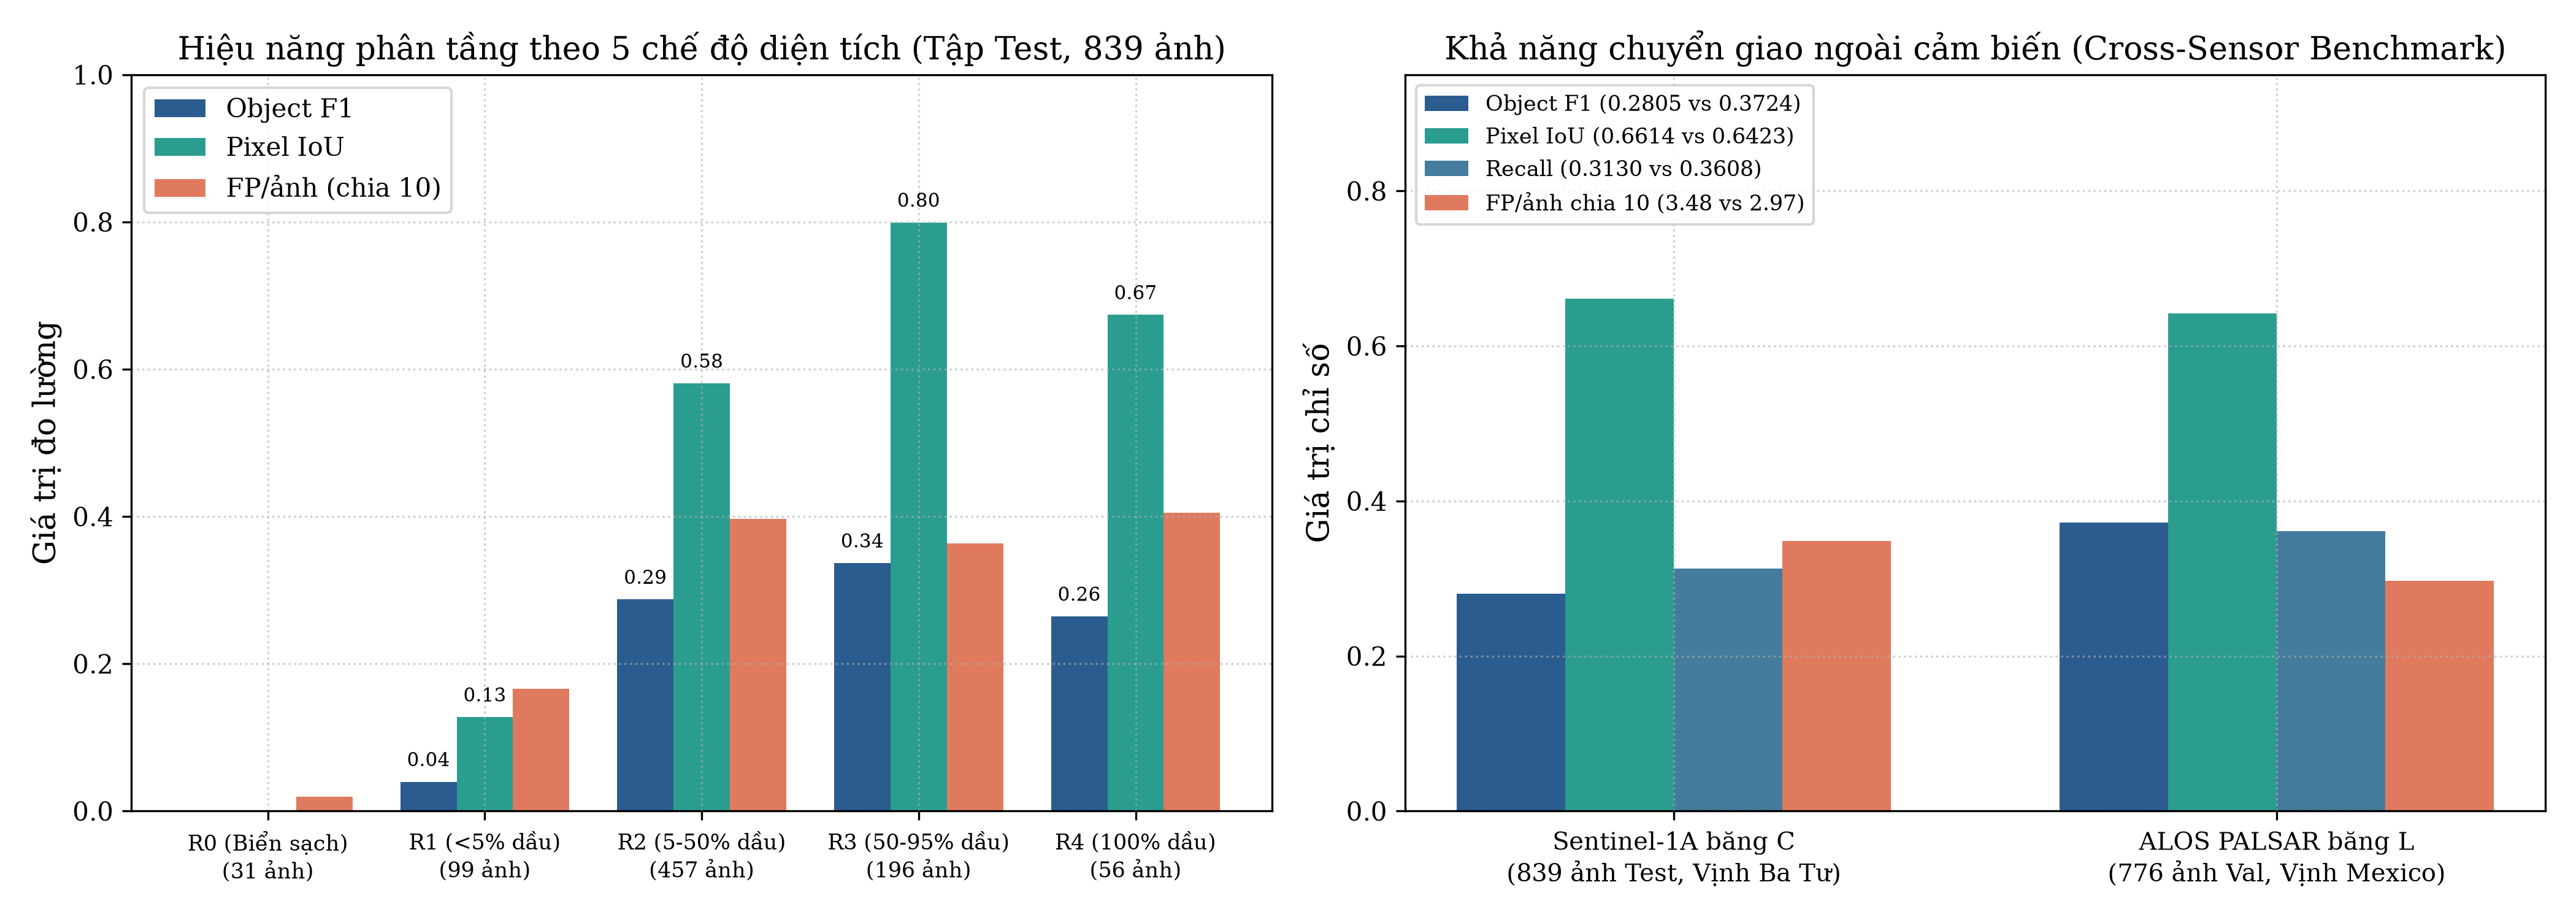
\includegraphics[width=\linewidth]{figures/fig8_regime_sensor_performance.png}
\caption{Hiệu năng phân tầng của mô hình đề xuất theo 5 chế độ diện tích dầu ($R_0 \to R_4$, bên trái) trên 839 ảnh Test Sentinel-1A và đối sánh khả năng chuyển giao ngoài cảm biến sang 776 ảnh ALOS PALSAR (bên phải).}
\label{fig:regime_sensor}
\end{figure}

\begin{table}[!t]
\centering
\caption{Chi tiết hiệu năng phân tầng của mô hình đề xuất (LinearSVM) theo 5 chế độ diện tích dầu ($R_0 \to R_4$) trên cả hai tập kiểm thử độc lập: 839 ảnh Sentinel-1A (băng C) và 776 ảnh ALOS PALSAR (băng L).}
\label{tab:regime_breakdown}
\resizebox{\linewidth}{!}{%
\begin{tabular}{lccccccc}
\toprule
\textbf{Chế độ diện tích} & \textbf{Số ảnh} & \textbf{TP} & \textbf{FP} & \textbf{FN} & \textbf{Object F1} & \textbf{Pixel IoU} & \textbf{FP / ảnh} \\
\midrule
\multicolumn{8}{l}{\textit{Tập kiểm thử cùng cảm biến Sentinel-1A (839 ảnh, Vịnh Ba Tư \& Biển Đông):}} \\
$R_0$ (Biển sạch, 0\% dầu) & 31 & 0 & 6 & 0 & N/A & N/A & \textbf{0.19} \\
$R_1$ (Vết dầu nhỏ, $<5\%$) & 99 & 9 & 164 & 271 & 0.0397 & 0.1276 & 1.66 \\
$R_2$ (Dải dầu trung bình, $5\text{--}50\%$) & 457 & 693 & $1\,814$ & $1\,624$ & 0.2873 & 0.5808 & 3.97 \\
$R_3$ (Dầu diện rộng, $50\text{--}95\%$) & 196 & 250 & 712 & 273 & \textbf{0.3367} & \textbf{0.7993} & 3.63 \\
$R_4$ (Ngập dầu toàn phần, $\ge 95\%$) & 56 & 44 & 227 & 18 & 0.2643 & 0.6738 & 4.05 \\
\textbf{Tổng hợp Sentinel-1A} & \textbf{839} & \textbf{996} & $\mathbf{2\,923}$ & $\mathbf{2\,186}$ & \textbf{0.2805} & \textbf{0.6614} & \textbf{3.48} \\
\midrule
\multicolumn{8}{l}{\textit{Tập kiểm thử ngoài cảm biến ALOS PALSAR (776 ảnh, Vịnh Mexico):}} \\
$R_0$ (Biển sạch, 0\% dầu) & 45 & 0 & 3 & 0 & N/A & N/A & \textbf{0.07} \\
$R_1$ (Vết dầu nhỏ, $<5\%$) & 113 & 36 & 223 & 359 & 0.1101 & 0.2274 & 1.97 \\
$R_2$ (Dải dầu trung bình, $5\text{--}50\%$) & 585 & $1\,360$ & $2\,034$ & $2\,165$ & 0.3931 & 0.6480 & 3.48 \\
$R_3$ (Dầu diện rộng, $50\text{--}95\%$) & 31 & 43 & 45 & 29 & 0.5375 & 0.8153 & 1.45 \\
$R_4$ (Ngập dầu toàn phần, $\ge 95\%$) & 2 & 2 & 0 & 0 & \textbf{1.0000} & \textbf{0.8827} & \textbf{0.00} \\
\textbf{Tổng hợp ALOS PALSAR} & \textbf{776} & $\mathbf{1\,441}$ & $\mathbf{2\,305}$ & $\mathbf{2\,553}$ & \textbf{0.3724} & \textbf{0.6423} & \textbf{2.97} \\
\bottomrule
\end{tabular}%
}
\end{table}

Bảng~\ref{tab:regime_breakdown} và Hình~\ref{fig:regime_sensor} phân tích chi tiết hiệu năng theo từng lát cắt dữ liệu trên cả hai cảm biến:
\begin{enumerate}
    \item \textbf{Phân tầng diện tích ($R_0 \to R_4$):}
    \begin{itemize}
        \item Ở chế độ biển sạch $R_0$, dù thuật toán Otsu luôn cắt ra các vùng tối giả trên nền biển đơn đỉnh ($754$ FP ứng viên trên 31 ảnh Sentinel-1A, tương đương $24.32$ FP/ảnh), bộ phân loại vùng LinearSVM đã loại bỏ $99.2\%$ số ứng viên này: chỉ còn tổng cộng $6$ vùng báo nhầm trên 31 ảnh Sentinel-1A (đạt \textbf{$0.19$ FP/ảnh}, khoảng tin cậy Bootstrap 95\% $[0.06, 0.35]$ FP/ảnh, trong đó $25/31$ ảnh sạch hoàn toàn $0$ FP và $6/31$ ảnh có đúng $1$ FP) và chỉ $3$ vùng báo nhầm trên 45 ảnh ALOS PALSAR (\textbf{$0.07$ FP/ảnh}, với $42/45$ ảnh đạt $0$ FP). Tuy nhiên, do cỡ mẫu $R_0$ trong bộ dữ liệu SOS khá nhỏ ($31$ và $45$ ảnh), kết quả này chưa đủ để ngoại suy trực tiếp sang kịch bản giám sát đại dương mở quy mô lớn (nơi $>99\%$ diện tích là biển sạch và mức $0.19$ FP/patch vẫn có thể sinh ra hàng trăm cảnh báo giả trên mỗi cảnh SAR nguyên vẹn nếu không có bộ cổng kiểm định đa đỉnh đứng trước Otsu).
        \item Ở chế độ $R_1$ (vết dầu nhỏ $<5\%$), Object F1 chỉ đạt $0.0397$ trên Sentinel-1A và $0.1101$ trên PALSAR do diện tích dầu nhỏ làm suy yếu sự tách biệt hai đỉnh của histogram toàn cục.
        \item Trên cả hai cảm biến, hiệu năng tăng mạnh từ $R_2$ sang $R_3$: trên Sentinel-1A, Object F1 đạt đỉnh ở $R_3$ ($0.3367$, Pixel IoU $= 0.7993$); trên PALSAR, $R_2$ (chiếm tới $585/776$ ảnh) đạt F1 $= 0.3931$ và $R_3$ đạt F1 $= 0.5375$ (Pixel IoU $= 0.8153$).
        \item Ở chế độ ngập dầu $R_4$ trên Sentinel-1A ($56$ ảnh), Pixel IoU vẫn đạt $0.6738$ nhưng Object F1 giảm xuống $0.2643$ ($4.05$ FP/ảnh) do hiện tượng vỡ hạt phân mảnh thành nhiều mảnh con không đạt $\IoU \ge 0.5$ cùng sự suy biến của nhánh fallback tính nền biển như đã phân tích.
    \end{itemize}
    \item \textbf{Đánh giá chuyển giao ngoài cảm biến (ALOS PALSAR):} Khi áp dụng mô hình LinearSVM đã đóng băng từ Sentinel-1A (băng C, phân cực VV) sang kiểm thử trực tiếp trên 776 ảnh ALOS PALSAR (băng L, phân cực HH) tại Vịnh Mexico, hệ thống đạt Object F1 $= 0.3724$, Pixel IoU $= 0.6423$ và tỷ lệ báo nhầm $2.97$ FP/ảnh. Phân tích phân bố chế độ trong Bảng~\ref{tab:regime_breakdown} giải thích rõ vì sao chỉ số tổng hợp trên PALSAR cao hơn Sentinel-1A: (i) Tập PALSAR tập trung tới $75.4\%$ số ảnh ở chế độ trung bình $R_2$ ($585/776$ ảnh) và hầu như không có các patch ngập dầu $R_4$ gây lỗi phân mảnh (chỉ có $2$ ảnh $R_4$ so với $56$ ảnh ở Sentinel-1A); (ii) Các vết dầu thô từ sự cố Deepwater Horizon có mật độ cao ($5.15$ đối tượng GT/ảnh so với $3.79$ ở Sentinel-1A) và độ tương phản bức xạ rõ nét hơn, giúp \texttt{Interior Recall} đạt $18.90\%$ (gần gấp đôi mức $10.48\%$ của Sentinel-1A). Kết quả này xác nhận rằng quy trình có khả năng chuyển giao trực tiếp sang tập ảnh chuẩn hóa $256 \times 256$ của cảm biến thứ hai trong bộ dữ liệu SOS, song cần lưu ý đặc trưng diện tích tỷ đối \texttt{area\_fraction} ($f_0$) vẫn phụ thuộc vào kích thước cửa sổ cắt patch và độ phân giải không gian vật lý của cảm biến.
\end{enumerate}


% Section 7: Conclusion
\section{Kết luận và định hướng tương lai}
\label{sec:conclusion}

Nghiên cứu này đã thiết kế, cài đặt từ đầu bằng NumPy và đánh giá thực nghiệm có kiểm soát một quy trình hai giai đoạn kết hợp giữa lọc đốm không gian, phân đoạn ngưỡng toàn cục và phân loại học máy theo vùng nhằm phát hiện vết dầu loang trên ảnh SAR đơn kênh. Bằng việc tính toán mô-men cục bộ của bộ lọc Lee MMSE trong thời gian $\mathcal{O}(HW)$ qua bảng tích phân và huấn luyện bộ phân loại LinearSVM tối ưu bằng thuật toán Nesterov Accelerated Gradient (NAG) trên không gian 8 đặc trưng vùng (cùng hệ số chặn bias tạo thành vector tham số 9 chiều), công trình đã cung cấp một cơ sở thực nghiệm minh bạch về cả hiệu quả giảm báo nhầm lẫn các giới hạn cấu trúc của phương pháp cổ điển trên bộ dữ liệu SOS.

Kết quả kiểm thử độc lập trên 839 ảnh Sentinel-1A (chứa $3\,182$ đối tượng dầu tham chiếu) và 776 ảnh ngoài cảm biến ALOS PALSAR ghi nhận các chỉ số định lượng chính xác như sau:
\begin{itemize}
    \item \textbf{Triệt tiêu cảnh báo sai ở giai đoạn phân loại vùng}: Khi so sánh có kiểm soát ở cùng cấu hình tạo ứng viên (Lee $7 \times 7, L=4$ + Otsu + $A_{\min} = 64$), bộ phân loại LinearSVM đã loại bỏ $76.6\%$ số vùng báo nhầm (cắt giảm $9\,572$ vùng tối giả, đưa tỷ lệ cảnh báo sai từ $14.89$ xuống $3.48$ FP/ảnh), đặc biệt giảm $99.2\%$ báo nhầm trên các ảnh biển sạch $R_0$ (từ $24.32$ xuống $0.19$ FP/ảnh, khoảng tin cậy Bootstrap 95\% $[0.06, 0.35]$, với $25/31$ ảnh đạt $0$ FP).
    \item \textbf{Cải thiện độ chính xác cấp đối tượng và cấp điểm ảnh}: LinearSVM nâng Precision từ $0.0753$ lên $0.2541$ (tăng $3.37$ lần) và nâng Object F1 từ $0.1220 \ [0.1124, 0.1328]$ lên $0.2805 \ [0.2652, 0.2980]$ ($\Delta\text{F1} = +0.1586 \ [+0.1474, +0.1706]$). Bộ phân loại giữ lại $97.8\%$ số đối tượng đúng do Giai đoạn 1 đề xuất ($996/1\,018$ TP), đạt độ thu hồi tổng thể $\text{Recall} = 0.3130$ trên toàn bộ $3\,182$ đối tượng Ground Truth. Về mặt diện tích điểm ảnh, hệ thống đạt Global Pixel IoU $= 0.6614$ trên toàn tập và Macro Pixel IoU trung bình từng ảnh đạt $0.577 \pm 0.261$ ($n = 814$).
    \item \textbf{Đánh giá ngoài cảm biến trên ALOS PALSAR}: Khi áp dụng trực tiếp mô hình đã khóa sang 776 ảnh ALOS PALSAR băng L mà không huấn luyện lại, quy trình đạt Object F1 $= 0.3724$, Global Pixel IoU $= 0.6423$ và tỷ lệ báo nhầm $2.97$ FP/ảnh ($0.07$ FP/ảnh trên 45 ảnh biển sạch $R_0$), phản ánh khả năng tương thích tốt trên các cảnh sự cố tràn dầu có độ tương phản cao ở chế độ diện tích trung bình $R_2$.
    \item \textbf{Hiệu năng tính toán}: Quy trình thực thi hoàn toàn trên CPU mất trung bình $50.2 \pm 14.7\text{ ms/ảnh}$ kích thước $256 \times 256$ (thông lượng đo trên 4 tiến trình song song), nhanh hơn phương pháp phân ngưỡng trực tiếp trên ảnh thô nhờ giảm hơn $72\%$ số thành phần liên thông cần xử lý.
\end{itemize}

Quan trọng hơn, phân tích đối chứng và giải phẫu lỗi xuyên suốt bài báo đã làm sáng tỏ bốn phát hiện khoa học cốt lõi về mặt phương pháp luận:
\begin{enumerate}
    \item \textit{Hiện tượng suy biến của trọng số Lee MMSE trên ảnh SAR nén 8-bit}: Trên các bộ dữ liệu đã qua tiền xử lý đa nhìn và lượng tử hóa 8-bit như SOS, hệ số biến thiên cục bộ $C_I^2 = v/m^2$ tại phần lớn các vùng đồng nhất đều nhỏ hơn nhiều so với ngưỡng phương sai nhiễu lý thuyết $1/L$ khi chọn $L \in \{1, 4\} \ll \text{ENL}_{\text{eff}}$. Điều này khiến trọng số $W(x, y) = \max(0, 1 - \frac{1/L}{C_I^2})$ bằng $0$ trên diện rộng và làm bộ lọc Lee $7 \times 7$ hoạt động tương đương thống kê với bộ lọc trung bình hộp Mean $7 \times 7$ ($\Delta\text{F1} = +0.0014$, khoảng tin cậy 95\% $[-0.0003, +0.0033]$ chứa 0).
    \item \textit{Sự lệch pha cấu trúc giữa nhãn huấn luyện Purity và thước đo Hungarian IoU}: Bộ phân loại vùng đạt F1 tới $80.74\%$ khi đánh giá theo nhãn tinh khiết ($\mathrm{Purity} \ge 0.50$), nhưng hơn một nửa số dự đoán dương tính bị tính là False Positive ở cấp đối tượng ($>1\,250 / 2\,215$ FP trên tập Validation) thực chất là các mảnh dầu thật bị phân ngưỡng Otsu cắt vụn khiến từng mảnh riêng lẻ không đạt ngưỡng ghép cặp 1--1 $\IoU \ge 0.50$ với mặt nạ GT nguyên khối.
    \item \textit{Nút cổ chai độ thu hồi và suy biến ước lượng nền ở chế độ ngập dầu}: Trần Recall của toàn hệ thống bị khóa bởi bước phân ngưỡng Otsu toàn cục ($\le 0.3199$, trong đó các vết dầu nhỏ nội vùng chỉ đạt \texttt{Interior Recall} $= 10.48\%$). Đồng thời, trên các patch ngập dầu ($R_3, R_4$), việc chỉ lấy các điểm ảnh ngoài ứng viên làm nền khiến ước lượng $\mu_{\text{bg}}$ bị thiên lệch về phía sáng và làm suy giảm hiệu lực của đặc trưng tương phản nền.
    \item \textit{Đa cộng tuyến đặc trưng và hạn chế cấp độ patch}: Đặc trưng \texttt{boundary\_gradient} ($f_6$) có tương quan đơn biến dương với nhãn dầu ($r = +0.3632$) nhưng nhận trọng số âm ($w_6 = -0.639$) trong mô hình LinearSVM do đóng vai trò biến ức chế (suppressor variable) trước sự cộng tuyến mạnh với độ lệch chuẩn nội vùng ($r = +0.8504$) và tương phản nền ($r = +0.6716$). Ngoài ra, việc dữ liệu gốc thiếu siêu dữ liệu cảnh chụp (scene ID) và độ phân giải vật lý khiến đánh giá hiện tại giới hạn ở cấp độ patch $256 \times 256$.
\end{enumerate}

Từ những kết luận thực nghiệm trên, các hướng phát triển tiếp theo được định hình rõ ràng:
\begin{enumerate}
    \item \textbf{Hợp nhất vùng hậu phân loại và đồng bộ hóa hàm mục tiêu}: Bổ sung bước gom cụm không gian (spatial region merging / morphological bridging) đối với các ứng viên lân cận cùng được dự đoán là dầu nhằm khắc phục hiện tượng phân mảnh đối tượng và thu hẹp khoảng cách giữa nhãn huấn luyện Purity với thước đo đánh giá Hungarian IoU.
    \item \textbf{Ước lượng tự động $\text{ENL}_{\text{eff}}$ và cổng kiểm định đa đỉnh (Bimodality Gate)}: Tự động ước lượng số lượt nhìn hiệu dụng từ vùng biển đồng nhất để hiệu chỉnh tham số $L$ cho bộ lọc Lee trên ảnh 8-bit, đồng thời tích hợp kiểm định thống kê đa đỉnh trước bước phân ngưỡng nhằm ngăn chặn việc ép cắt Otsu trên các khung ảnh biển sạch ($R_0$) hoặc ngập trọn dầu ($R_4$).
    \item \textbf{Mở rộng quy mô cửa sổ lọc và chuẩn hóa theo siêu dữ liệu cảnh gốc}: Khảo sát mở rộng kích thước cửa sổ lọc ($9 \times 9, 11 \times 11$) kết hợp với các mô hình đề xuất ứng viên đa tỷ lệ (như CFAR thích nghi hoặc mạng phân đoạn nhẹ) trên dữ liệu Sentinel-1 Level-1 GRD gốc có đầy đủ tọa độ địa lý để đánh giá độc lập theo từng cảnh chụp (scene-level split).
\end{enumerate}


% --- Bibliography ---
\bibliographystyle{elsarticle-num}
\bibliography{references}

\end{document}

